% !TEX TS–program = pdflatexmk
%%%%%%%%%%%%%%%%%%%%%%%%%%%%%%%%%%%%%%%%%%%%%%%%%%%%%%%%%%%
% EPFL report package, main thesis file Goal: provide formatting for theses and
% project reports Template's Author: Mathias Payer <mathias.payer@epfl.ch>
% Thesis's Author : Arnaud Pannatier <arnaud.pannatier@epfl.ch>
%%%%%%%%%%%%%%%%%%%%%%%%%%%%%%%%%%%%%%%%%%%%%%%%%%%%%%%%%%%
\documentclass[a4paper,11pt,oneside]{report}
% Options: MScThesis, BScThesis, MScProject, BScProject
\usepackage[MScThesis]{EPFLreport} \usepackage{xspace}
\usepackage{array}
\usepackage{rotating}
\usepackage{booktabs}
\usepackage{placeins}
\usepackage{array}
\newcommand{\PreserveBackslash}[1]{\let\temp=\\#1\let\\=\temp}
\newcolumntype{C}[1]{>{\PreserveBackslash\centering}p{#1}}
\newcolumntype{R}[1]{>{\PreserveBackslash\raggedleft}p{#1}}
\newcolumntype{L}[1]{>{\PreserveBackslash\raggedright}p{#1}}
\usepackage{arydshln}

\title{A Control Plane in Time and Space for Locality-Preserving Blockchains}
\author{Arnaud Pannatier}
\supervisor{Cristina Basescu}
\adviser{Prof. Bryan Ford}
%\coadviser{Second Adviser}
\expert{\color{red}The External Reviewer\color{black}}

\newcommand{\sysname}{FooSystem\xspace}

\begin{document}

\maketitle 

\maketoc

%%%%%%%%%%%%%%%%%%%%
\chapter{Introduction}
%%%%%%%%%%%%%%%%%%%%

%% Presentation and setting
Distributed ledgers are a becoming more and more used as they provide
independence to a central authority, anonymity, security of transaction,...
Some distributed ledgers as Bitcoin \cite{Nakamoto2009} managed to get a lot of
popularity for various reasons. However they still are subject to some
weakness. The purpose of this work is to advances the research concerning two
of them. The first one is the time to confirm a transaction. 
Indeed, in Bitcoin \cite{Nakamoto2009}, validating a transaction can take around one
hour, because it takes around ten minutes to validate a block, and it needs
around six blocks to be convinced with a high probability that the ledger won't
be forked, and the transaction invalidated. This might be okay for some
transactions of great value. For example if somebody is buying a car using
Bitcoin, this person might agree to wait one hour so that its transaction is
validated. However if somebody wants to buy its daily coffee using bitcoin, it
might be a bit annoyed with this waiting time. The other problem is World War
III scenarios. If a third World War occurs, splitting the world in two, one can
expect that the communication between the two sides might be cut. This is a
problem for regular distributed ledger as it will lead to forks that cannot be
resolved at the end of WWIII.  This work is part of a bigger project called Nyle
[\autoref{fig:Nyle}], which uses the idea of locality to solve these problems.
The idea is to replicate the system along regions of different sizes, from
local (e.g.  Switzerland, London) to global. With this idea a transaction can
be validated in a local region first, but it still possible to wait for global
validation if needed. Most of the time a transaction validated locally will be
validated globally as well, but in some case, when propagating the information
to the global regions, some transactions might be invalidated to avoid double
spending. For big transactions, people might prefer to wait for the global
confirmation. But if one wants to buy its daily coffee, local validation might
be enough for the merchant, especially if he knew already the person. For
World War III Scenarios, Nyle offers a solution as well, indeed if a global
partition occurs, the system replicated in smaller regions that are not split
by a partition can still continue working flawlessly. 

\begin{figure}[!h]
\centering
\includegraphics[width=400pt]{figures/Nyle}
\caption{Sketch of Nyle: The blockchain is replicated across region}
\label{fig:Nyle}
\end{figure}

%% Main Challenge
Nyle's distributed ledger is maintained by nodes that are spread over the world.
Clients will then ask the nodes to proceed their transactions or other
requests. Nodes are participating to a different number of regions. A first
challenge is to draw these regions in a satisfactory manner. A second problem
is \textit{open-membership} : it should be possible for anybody with a
sufficient computational power and a good connection to maintain a node of the
system. This allows the system to be distributed. The challenge with
\textit{open-membership} is that there should be a way to know the participants
of the system if one wants to have a consensus.   A second challenge is that
nodes can join, leaves or move in the system at any moment. This might not be a
problem for classic distributed ledger as Bitcoin \cite{Nakamoto2009}, as its
protocol only take in account the computational power that is in the system at
a given time. But as Nyle is locality-based, this might lead to additional
challenges, each corresponding to the different actions possible : joining,
leaving and moving. For joining nodes, consider the case where there was only a
few nodes spread along a big region, for example Western Europe, and after a
while a large number of new nodes wants to join in that part. If the region
stays the same, this might lead to some problems, indeed the consensus would
take more time and the liveness could not be guaranteed. Furthermore for a
region of this size, the probability of a partition is relatively important.
One might want that in this case, additional regions, corresponding for example
to country might be created. This leads to the idea that the regions should be
able to adapt depending to node membership.  If nodes leave the system, this
might lead to problems as well. Indeed in the inverse situation as before,
after a while some regions might not contains any node that are maintaining the
system. To avoid this situation, one might want to adapt the region when nodes
leaves to guarantee that a sufficient number of nodes are in a region at any
time. Moving nodes are creating problems as well, if the region assignment is
fixed but the nodes are moving, a node drift appart after a while far away from
the region it was assigned to. This might take a while, but one can imagine the
situation where a lot of nodes have moved far away from their original
position. In case of a global partition, this can lead to the failure of even
small regions, that is one problem that one wants to avoid in Nyle. Therefore
the regions should be adapted with the movement of the nodes. 

%% Related Work Is Insufficient
Most of this work is based on the CRUX \cite{Basescu2014}, which introduces the
algorithm that allow to draw regions based on compact graph theory and which is
described in more detail in  \autoref{chap:Background}. The existing work on
Nyle was done by Maxime Sierro and Cristina Basescu \cite{Sierro2019} which
proposes a first implementation of Nyle building on the top CRUX
\cite{Basescu2014} but focusing directly how to improve the storage of the
transactions and the tree structure of the regions. This works builds directly
upon the existing work, but is slightly orthogonal, as the Controle Plane is
not directly linked to the replicated blockchain.  A  second work on Nyle was
done by Sabrina Kall \cite{Kall2019}, which was proposing a way of checking
efficiently the location of a node and to assert if nodes were lying about the
location where they claimed to be. There is a current work on the
Interplanetary-File System (IPFS) \cite{Michel2019}, that is based on CRUX as
well but with the purpose to create a locality-aware overlay to speed the
system up, but it is not directly related to blockchains. The rest of the
related work is described in the next chapter \autoref{chap:RelatedWork} and is
mostly orthogonal to the current approach : some other solutions to speed the
validation of transaction are Bitcoin \cite{Nakamoto2009}, Byzcoin
\cite{Kogias2016}, Omniledger \cite{Kokoris-Kogias2017},  DFINITY
\cite{Hanke2018}, Monoxide \cite{Wang2019} and Stellar \cite{Lokhava2019}, but
they don't use the concept of the locality for this purpose. 

%% Description of the Approach
This work was structured in the following manner : first a simple version of
the control plane was designed \autoref{chap:Design}, which splits the time into
epochs and take as an assumption that the system is fixed during one epoch. A
protocol is proposed and discussed and the threat analysis is done. Based on
its implementation and performance analysis some drawbacks are put in light.
Then a series of strawman models try to correct some of these drawbacks and are
analyzed as well \autoref{chap:Improvements}. The first one is called "Locarno
Treaties" and will try to keep the system coherent from one epoch to the next.
The next one is called "Fog of the war", and try to reduce the need for
communication between nodes. The last and the most complex consider the
interactions of the nodes as a space-time graph and try to build upon the
existing patterns that appears in these graphs to solve the problem of control
plane. 

%% Why it is needed.
%% Already discussed in Main challenges so it is merged with the next

%% Thesis Statement
This works proposes \textbf{A Control Plane in Time and Space for
Locality-Preserving Blockchains}. This control plane for Nyle is needed to
ensure to have a \textit{open-membership} and to solve the problems of World
War III scenarios and to allow regional validations. The series of strawman
models improving the simple control plane lead to the use of Space-Time graphs
that allowed to improve the existing design. 

%% Results 

%%My  Contribution

%%%%%%%%%%%%%%%%%%%%
\chapter{Related Work} \label{chap:RelatedWork}
%%%%%%%%%%%%%%%%%%%%
This work builds upon several other works that are linked to the domains of
blockchains and locality. Nyle proposes a decentralized cryptocurrency using
different strategies than Bitcoin \cite{Nakamoto2009}, Byzcoin \cite{Kogias2016},
Omniledger \cite{Kokoris-Kogias2017}, DFINITY \cite{Hanke2018}, Monoxide
\cite{Wang2019} and Stellar \cite{Lokhava2019}.But it used them as a source of inspiration
and share some aspects with theses general cryptocurrencies.  It is
somehow orthogonal to them because it can use any of theses cryptocurrencies as
an underlying system and enhance them using the idea of locality to add some
partition-resistance to them. 

Some concepts are directly inspired from these works. The Sybil-resistance
scheme used in the registration system is directly inspired from DFINITY
\cite{Hanke2018}, using \textit{endorsement} in the general way, which can be
in practice replaced by any Sybil-resistance scheme like Proof-of-Work
\cite{Nakamoto2009}, Proof-of-Stake \cite{wood2014ethereum}, or even
Proof-of-Personhood \cite{Borge2017}. In particular this work tries to solve
some drawbacks of traditional cryptocurrencies like \cite{Nakamoto2009},
solving the problem of the waiting time for validation by using region
validation and making it resistant to WWIII scenarios. Byzcoin
\cite{Kogias2016} and Omniledger \cite{Kokoris-Kogias2017} gives another
interesting solution to accelerate the validation, but their results are
orthogonal to this research. Stellar's solution for \textit{open-membership}
\cite{Lokhava2019} is based on a quorum, allowing each node to trust a subset
of other nodes of its choice. It is an elegant solution and permits to validate
transactions fast and securely. A certain complexity seems to be added both in
theoretical part and practice, this justifies why  a similar approach was not
followed. However the idea to allow nodes to have a different view of the
system is at the core of one of the improvements of this work.

Omniledger \cite{Kokoris-Kogias2017}  and Monoxide \cite{Wang2019} uses
sharding to increase performance.  Sharding splits the system in random
committee that allow the fastest processing of the transaction. This not
directly related of what is done in this work, as even if the system is split
in different parts, it is not done randomly but based on the locality, and the
system is replicated in all the regions. However, cryptocurrencies using shards
can still be used as an underlying system of Nyle, enhancing the performance of
the partition-resistant blockchain system created by this means.

This work is directly related to the locality-preserving algorithms developed
in CRUX \cite{Basescu2014} and compact-graph algorithms \cite{Thorup2005}.
These are described in detail in \autoref{chap:Background}. There is a class of
algorithm that uses the idea of locality in a different manner. For example
Geo-DNS \cite{Katz-bassett2006} or IP Anycast \cite{Abley2006} use the idea of
locality to shorten the path for the packets, connecting the servers via the
closest path. Replication is often used to guarantee integrity of the stored
information \cite{find-paper-replication}. In CRUX \cite{Basescu2014} and Nyle
regional replication of the system is used to create partition-resistance, and
in Nyle it can be used to allow region validation.

Classic consensus algorithms as PAXOS \cite{Lamport2000}, PBFT
\cite{Castro1999} were used as an inspiration to develop some parts of the
theoretical algorithm. In practice, and for efficiency, this work use BlsCoSi
\cite{Boneh2018} that is much more efficient, using trees for communication.
BlsCoSi \cite{Boneh2018} is still prone to some drawbacks in case of successive
view-changes, it could be improved using a different algorithm such as HotStuff
\cite{Yin2018} which solves the problem of view change using a third round of
communication. %% TODO VALIDATE. 

This works uses a distributed public algorithm for the source of randomness
like Randhound \cite{Syta2016}. Each node will use this source to draw a random
level.  The way it is used is described in detail in the next section. 


%%%%%%%%%%%%%%%%%%%%
\chapter{Background} \label{chap:Background}
%%%%%%%%%%%%%%%%%%%%

%%%% Plan
% - Crux (??)
% - Nyle (7-8p) - General description - What is already implemented - Next
%   steps
% (motivation for the control plane)
%%%%%%%%%%%%%%%%%%

This Master Thesis is part of a biggest project that concerns
locality-preserving systems. In particular, it builds upon
CRUX \cite{Basescu2014} and is part of Nyle. This section describes the two
different projects. 

\section{CRUX}

%%%% General Presentation
% - Solution to partition
% - General idea
% - Small Overhead
% - Generality 
% - CAP Theorem
%%%%%%%%%%%%%%%%%%
\subsection{Description}
CRUX \cite{Basescu2014} introduces a smart way of dealing with partitions in
decentralized systems. The purpose is the following : partitions occur in
decentralized systems. But one can maybe try to find a solution to reduce their
effects on the global system. For example, if a partition occurs, there is no
reason that nodes that are functioning in the same side of the partition should
stop working because of the partition. 

The general idea is that a system can be replicated at different scales, from
local (cities, region) to global.  With the additional property than each
replicated system will continue to work correctly if no partition splits it. If
a global partition occur, then the global region might not work, but all the
replicated system in local regions will still continue working. This is a
direct solution to the previously mentioned problem : nodes working on the same
of the partition will continue to work.

Obviously, this solution comes with an overhead, as the system should be
replicated in all the regions. But there are some ways of reducing this
overhead, in a way that it stays reasonable and that the resistance to
partition is maintained. To reduce this overhead, CRUX algorithm for regions
creation \cite{Basescu2014} presented below ensure that the proper number of
regions is created in a manner that the number of regions created induce a
reasonable overhead and that the partition resistance stays efficient. If CRUX
\cite{Basescu2014} is used for a specific system, overhead can be even more
reduced:  as the systems are replicated in every region, most of the data is
replicated as well. So one might actually dig inside the specification of one
system and manages not to store twice the same data. But this overpass a bit
the goal of CRUX \cite{Basescu2014}, which wants to be the more general
possible. 

Indeed, the force of CRUX \cite{Basescu2014} is that it is applicable to any
distributed system, as no particular hypothesis on the system is made. It only
starts from one simple idea : one system can be replicated at smaller scale to
ensure partition resistance. 

% TODO : do more research on that.
A note should be made about the CAP-theorem. Recall that this theorem states
that no system can be consistent, available and partition-resistant at the same
time. It seems that this solution is adding partition tolerance to available
and consistent system. Thus leading to the violation of the theorem. But it is
not exactly the case, as the enhanced system only ensure that nodes can still
work in the same side of a partition. The regions split by a partition are not
working anymore. Even if the system can still work on the same side of a
partition, it's not totally partition resistant.

%%%% Common Tools
% - Approximation distance oracle
% - Bunch
% - Cluster
% - ARA 
%%%%%%%%%%%%%%%%%%
\subsection{Common Tools} \label{sec:common-tools}
This section describes how to create the
regions that are used to replicate the system. These regions are used by Nyle
as well, therefore we will describe it in detail. These regions are called
\textit{Available Responsive Areas} (ARA), in each region a copy of the replicated
system is deployed. To create these regions each node will participate first at
a lottery. Each node starts at level 0. Then each node go to the next level
with a given probability $P$. This
procedure is repeated at each level, and is stopped when no nodes are promoted
to the next level. This first empty level is called $K$. Then each node can
compute two quantities that will be necessary to create \textit{ARAs} : their
bunch and their cluster. 

\begin{table}[] 
\centering
\begin{tabular}{rrrrr}
& 100 & 200 & 500 & 1000 \\ \hline
\multicolumn{1}{r|}{0} & 90  & 180 & 450 & 900  \\
\multicolumn{1}{r|}{1} & 9 & 18  & 45  & 90   \\
\multicolumn{1}{r|}{2} & 1   & 2   & 5   & 9 \\
\multicolumn{1}{r|}{3} & 0   & 0   & 0   & 1
\end{tabular}
\caption{Example of lottery with $P = 0.1$ where $k= 3$ for $N= 100,200,500$
and $4$ for $N = 1000$.The columns represents the number of nodes and the row the levels. }
\label{example-lottery}
 \end{table}
 
\begin{figure}[!h] 
\centering
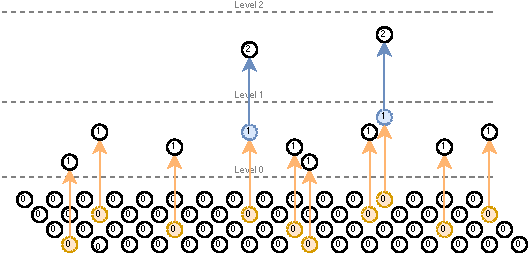
\includegraphics[width=400pt]{figures/Lottery-Standard}
\caption{Sketch of the Lottery process, nodes goes from one level to the next with probability $P$}
\label{fig:ClusterBunch-Bunch}
\end{figure}

\paragraph{Bunch} A node can compute its bunch in the following manner. It
looks at every other nodes by order of distances in ascending order and
includes it in its bunch if its level is not smaller than the one it encounters
so far, including its own level [\autoref{ClusterBunch-Bunch}]. 

\begin{figure}[!h] 
\centering
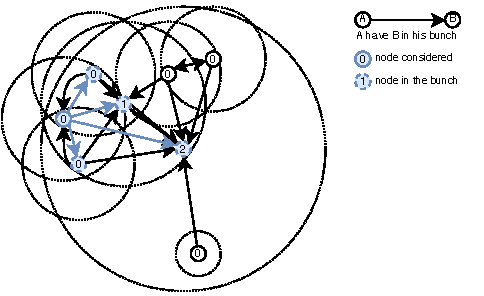
\includegraphics[width=250pt]{figures/ClusterBunch-Bunch}
\caption{ The bunch of the node is depicted in blue. }
\label{fig:ClusterBunch-Bunch}
\end{figure}

\paragraph{Cluster} A cluster is a complementary concept. The cluster of node
$A$ is defined as the set of other nodes that have $A$ in their bunch [\autoref{ClusterBunch-Cluster}]. 

\begin{figure}[!h] 
\centering
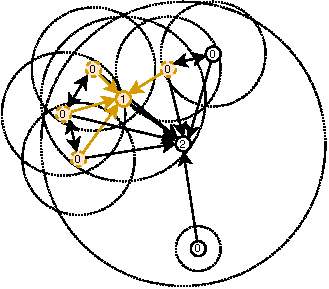
\includegraphics[width=250pt]{figures/ClusterBunch-Cluster}
\caption{ The cluster of the node is depicted in orange. }
\label{fig:ClusterBunch-Cluster}
\end{figure}

The smallest region radius $R_{min}$ is defined for the whole system. Each node
will construct $ARAs$ around itself starting at $R_{min}$ and doubling the
radius at each time. It stops at the first $ARA$ that is covering its entire
cluster. 

By the lottery, most nodes will be level-zero nodes. Therefore their cluster
supposed to be small, conducting to the creation of a small number of $ARA$s.
The small number of nodes that are at level $K-1$ will have every other nodes
in their cluster by construction. This means that there will be at least one
$ARA$ that covers the whole system. 

%%%% Nyle
%  - Problems it solves - Link with CRUX - Environment - Type of Blockchain 
% - What is already implemented 
% - Next steps. 
%%%%%%%%%%%%%%%%%%%%%%%%%%%%%
\section{Nyle}

Nyle is cryptocurrency that uses locality to answer some classical problems of
a blockchain systems. Two main problems are addressed: WWIII scenarios and
approval time for a transaction.
 
\paragraph{WWIII Scenarios} \label{WWIII} In case of a WWIII, we can expect to have
at least a long-lasting partition that will split the system in two. This is a
problem for classical cryptocurrencies like \cite{Nakamoto2009}, because for a
block to be approved, the users are supposed to wait to have a global
consensus. This consensus will not be reached with a long-lasting partition and
therefore it will create problems for classical cryptocurrencies. Nyle solves
this issue by design using locality.

\paragraph{Approval Time for a Transaction} \label{approve_time} Another issue
with waiting global consensus is that it usually takes a long time. If a
customer wants to use a cryptocurrency in a daily life, the nodes should be 
able to validate (at least partially) a transaction relatively fast. The
solution provided by Nyle use locality again: with Nyle a transaction is
validated at different geographical levels, and it is up to the customer to wait a local, or
global validation for a transaction. For small transaction, for example for
buying a coffee, the customer might agree to only have local validation. For
bigger transaction he might wants to wait a bit longer to have global
validation.

\subsection{Description}

Nyle uses ARA as the representation of one region. In each of these regions
there will be a copy of the same system, in the case of Nyle the system is a
blockchain. So each region will have its own blockchain and validate all the
transactions between the nodes that are included in it. Some nodes can be
included in different regions, and they will send their transactions to all the
regions they are part of. Which ensure that each blockchain will be updated
each time there is a transaction that concerns one of its nodes.

The big difference between CRUX \cite{Basescu2014} and Nyle is that the purpose
of CRUX \cite{Basescu2014} is to work in environments where machines are
relatively "stable" which means that they are not supposed to churn or to crash
often, and more, where the machines are not supposed to move. This is not the
case for Nyle : if we have a cryptocurrency, we can expect to have malicious,
deficient and/or moving nodes.  This will add some difficulties that will be
managed by the protocol.

Each region will have its own blockchain, in Nyle the choice for the blockchain
will be chosen between Omniledger \cite{Kokoris-Kogias2017} or ByzCoin
\cite{Kogias2016}. But it can be generalized to any kind of blockchain.

\subsection{What is already implemented for Nyle} 



\paragraph{CRUX algorithm for region creation} 
We already have an algorithm for drawing regions.

\paragraph{Block storage on node} As each node will participate in
different regions (from very local to world-wide), it will need to store the
blockchain for all of these regions. We have a method that reduces the
redundancy, by only storing the hash of a block instead of the full block at
each level. 

\paragraph{Proof-of-Location} We already have a protocol for controlling
the distance from a new node to the rest of the nodes. And that assures no one
cheats by giving false distances. 

%%%%% TODO : add general description 
%%%%% Motivation
% - Already have a system working for non-byzantine no-churn system 
% - Dealing with these problems can be done by dealing nodes insertion,
            %   deletion and moving.
% - If we solve that then we can return to the previous system and everything
            %   should be working
%%%%%%%%%%%%%%%
\subsection{Purpose of this project : Motivation for a control plane}

CRUX \cite{Basescu2014} proposes a system that is working in a stable system
(with low-churn) and where nodes do not move too much. As this situation
corresponds to some systems like wide-area database, ... It is definitely not
the case of a cryptocurrency.  For these kind of system, one can expect to have
at least some churn, some moving nodes and some adversarial nodes.  If the
system has a precise protocol for dealing with nodes entering, leaving and
moving in the system, then the problem of the evolution of the system is
solved. Indeed the churn phenomenon can be described as some nodes leaving the
system and optionally reentering later. 

Therefore the purpose of the control plane will be to deal with the evolution
of the regions that follows the evolution of the nodes in the system. Once that
problem is solved, the blockchain can be replicated in the evolving region and
the strategy will be the same as in CRUX \cite{Basescu2014}. Thus this project
introduce a control plane, that is in charge of the evolution of the nodes in
the system. In particular, it will be in charge of dealing with the nodes
joining, leaving and moving in the global system. If the blockchains is
replicated in all the regions, the control plane will be global. 

%%%%%%%%%%%%%%%%
\chapter{Design} \label{chap:Design}
%%%%%%%%%%%%%%%%

%%%%%%%%% 
%  - Problem definition (Hypothesis, Goals, ...) (2-3p) 
%%  - Hypothesis on the threat model
%  - First version: Simple Control Plane (15-20p ?) 
%%  - Graphs: Control flow, Protocol flow trough time 
%%  - Tools: Description of each subprotocols 
% %%%(consensus via Blscosi, gossips protocols, ...). 
%%   - Discussion
%%%%  - Advantages, prove that it fulfils the goal
%%%%%%  - Graph of difference between system without control plane and with. 
%%%%  - Drawback (evaluation of computational, memory and communication costs)
%%%%%%  - With graphs
%%  - Security  Analysis 
%%%%% - 2-3 scenarios illustrating malicious behaviors (written and/or with implementation)
%%%%%%%%%%%%%%%%%%%%%%%%%%%%%%%%%%%%%%%%%%%%%%%
This part will describe the design of the Control Plane, which has the mission
to solve the problem of node insertion, deletion and movement inside the
system. Allowing to use a CRUX region creation algorithm in an environment
with churn. 

\section{Problem definition}
%%%%%%%%%%%%%% Problem definition
%% Hypothesis : 
%%   - one-to-one communication
%%   - synchrone network
%%   - Correlation between pings and distances
%%   - Nodes are malicious
%%   - Adversary can delay communication
%%%%%%%%%%%%%%%%%%%%%%%%

\subsection{Hypothesis} Three hypotheses are made on the network. First it
assumes an internet-like network with one-to-one communication. Each node is
able to contact any other nodes. The network is supposed to be synchrone. This
means that every message sent by a node to another will arrive in order, and
that a message that is sent will be received within a given window of time. The
third hypothesis is made on the geometry of the network. It states that for
small pings (under 100ms) the ping time is actually correlated with the
distance between two nodes. This is the case for the Internet network
\cite{Seibert2014}. On this result we build the locality properties of the
system. 


%%%% mostly copied from
% https://docs.google.com/document/d/1xz1jTphKqxxkAucdh_oOqsFXH147Cjlzcnjmt-yx-f8/edit#heading=h.aq4k1vxbt0t0
\section{General Presentation}

The Control Plane is composed of five different components [FIG.
\autoref{fig:modules}], each necessary to solves different part of the problem. It
needs a membership component, to define precisely which nodes are in the system
at any time. It needs a locality component which gives the distance between two
nodes in the system. Then it needs a region management component, which will
draw the regions based on the membership and the locality. The time will be
split into epochs, a component is in charge of dealing that aspect. And
finally, the control plane is in charge of answering some requests linked to
the location and presence of the nodes in the system. Each will be described in
detail below. 

\begin{figure}[!h]
\centering
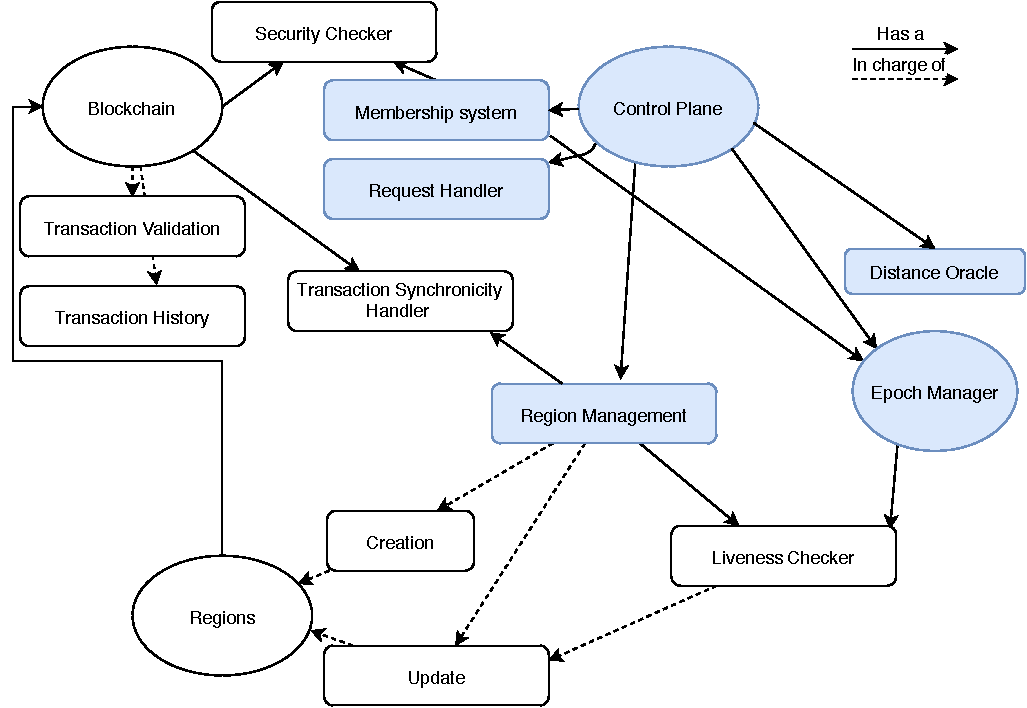
\includegraphics[width=400pt]{figures/Nyle_components}
\caption{List of modules of Nyle.  \color{red} TODO : REDO \color{black}}
\label{fig:modules}
\end{figure}

\subsection{Membership Component}

At each epoch, a registry contract containing a summary of all participants is
created. Registration use \textit{endorsement} (for example solution to a proof-of-work
problem). This system will be global. Nodes can ask the participants of the
system to know the identity of other nodes. To validate a new contract it
should be signed by the majority of the nodes of the previous epoch.

\subsection{Locality Component}

The role of the locality component is to give all pairwise latencies between
nodes of the system. We assume it already exists (distance oracle), or it can
be computed by nodes. In the first model all pairwise latencies is computed
between each node and every node agree on them via consensus. 
 
\subsection{Region Component} This component is used to create and update
regions. This part will be based on CRUX. At each epoch CRUX is run based on
the new registration, and regions are created.
 
\subsection{Epoch Component} The epoch manager is linked to the membership
system (we allow to change membership at the beginning of one epoch). New nodes
can join at the beginning of one epoch. If nodes have moved, the region
component will change or maintain their assignment at the beginning of one
epoch. If nodes have crashed, they won't be able to join for the next epoch and
will therefore leave the system.

Epochs happen at a defined rhythm (e.g. one day). This frequency can be
shortened to ensure that nodes that want to join do not wait too long, or made
longer if one wants regions not to be redrawn too frequently. 

\subsection{Request Handler} The control plane is the right part to get
requests as it is aware of the nodes location and region assignment. It will be
in charge of answering the request for nodes assignment and nodes location. 

\begin{figure}[!h] 
\centering
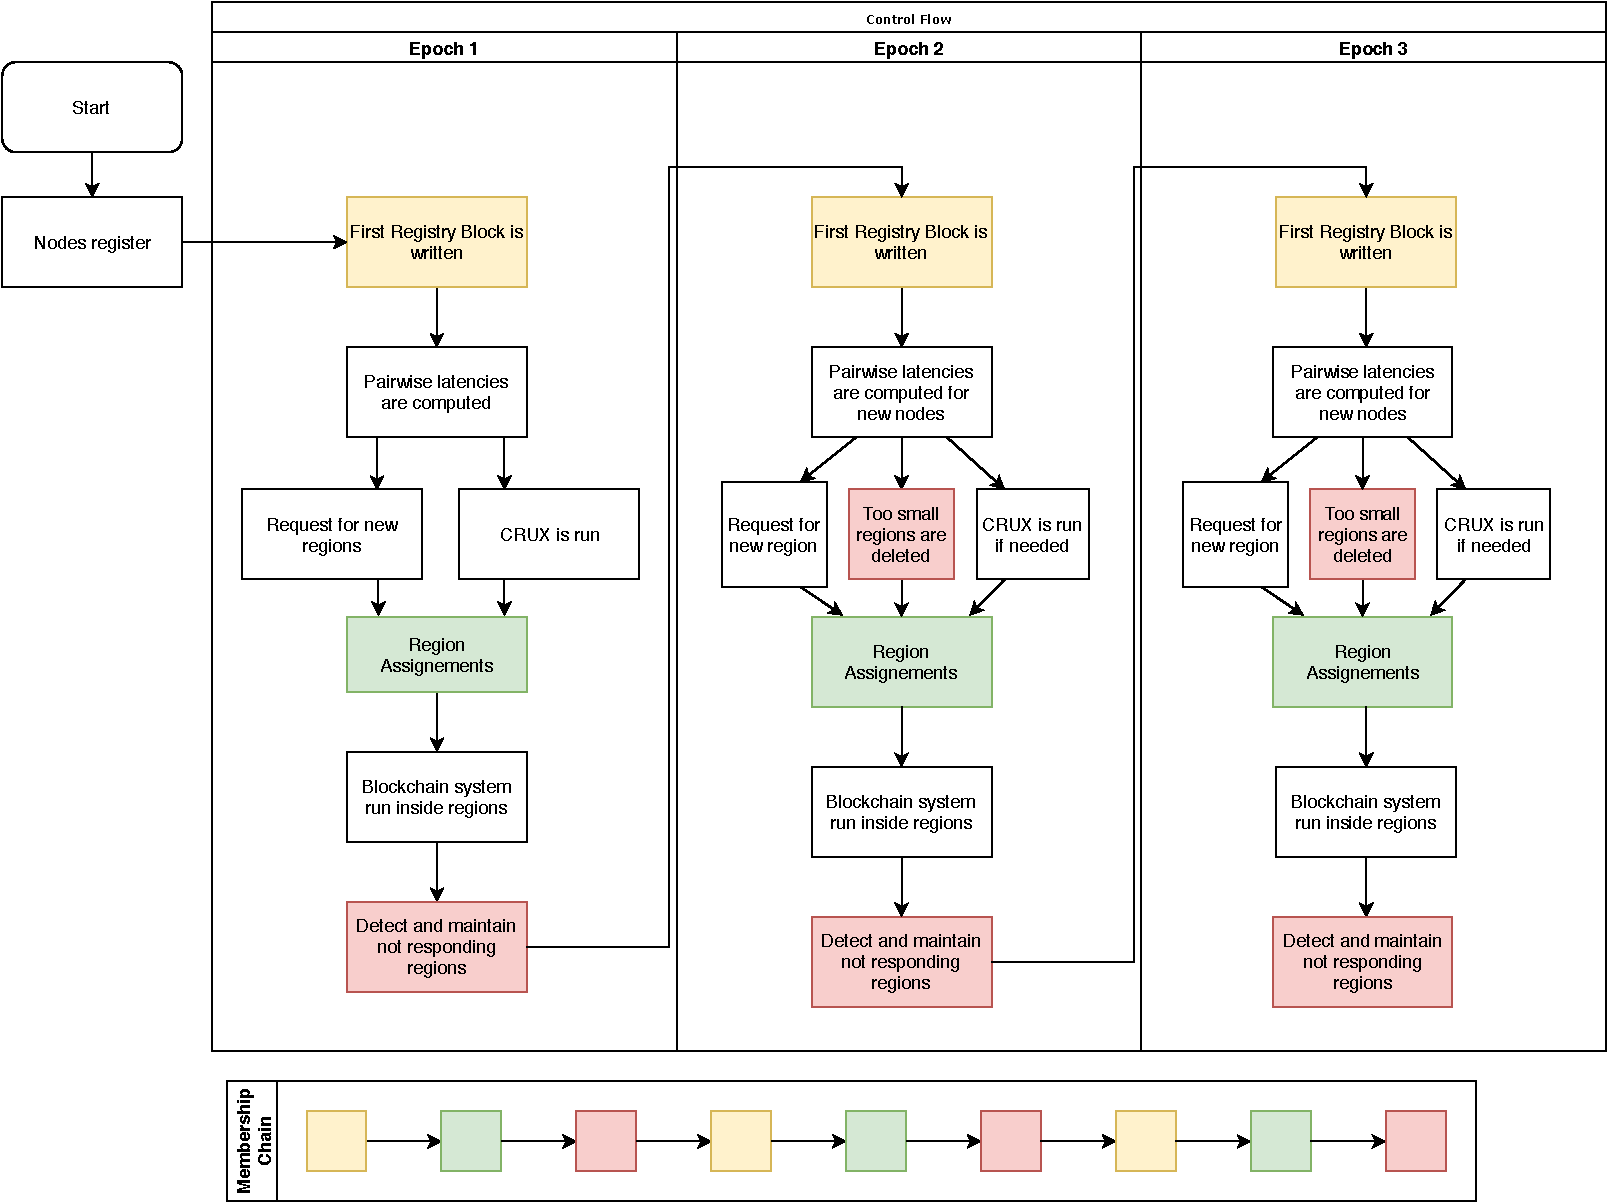
\includegraphics[width=400pt]{figures/Nyle_controlflow}
\caption{General control Flow of Nyle. \color{red} TODO : REDO \color{black}}
\label{fig:controlflow}
\end{figure}

\section{Simple Control plane} This version presents the first
version of the Control Plane. In which most of the work is done on the
membership component. At each epoch nodes can join if they manage to get an
approval from the members of the previous epoch. The locality component in this
model is brute force : every node computes its pings to every other nodes and
consensus is made on that information. The region component in this model is
simple : based on the registration, and the pings, CRUX is run at each
epoch. Redrawing the map of the entire system. 

\subsection{Membership Protocol}

\begin{sidewaysfigure}[!h]
\centering
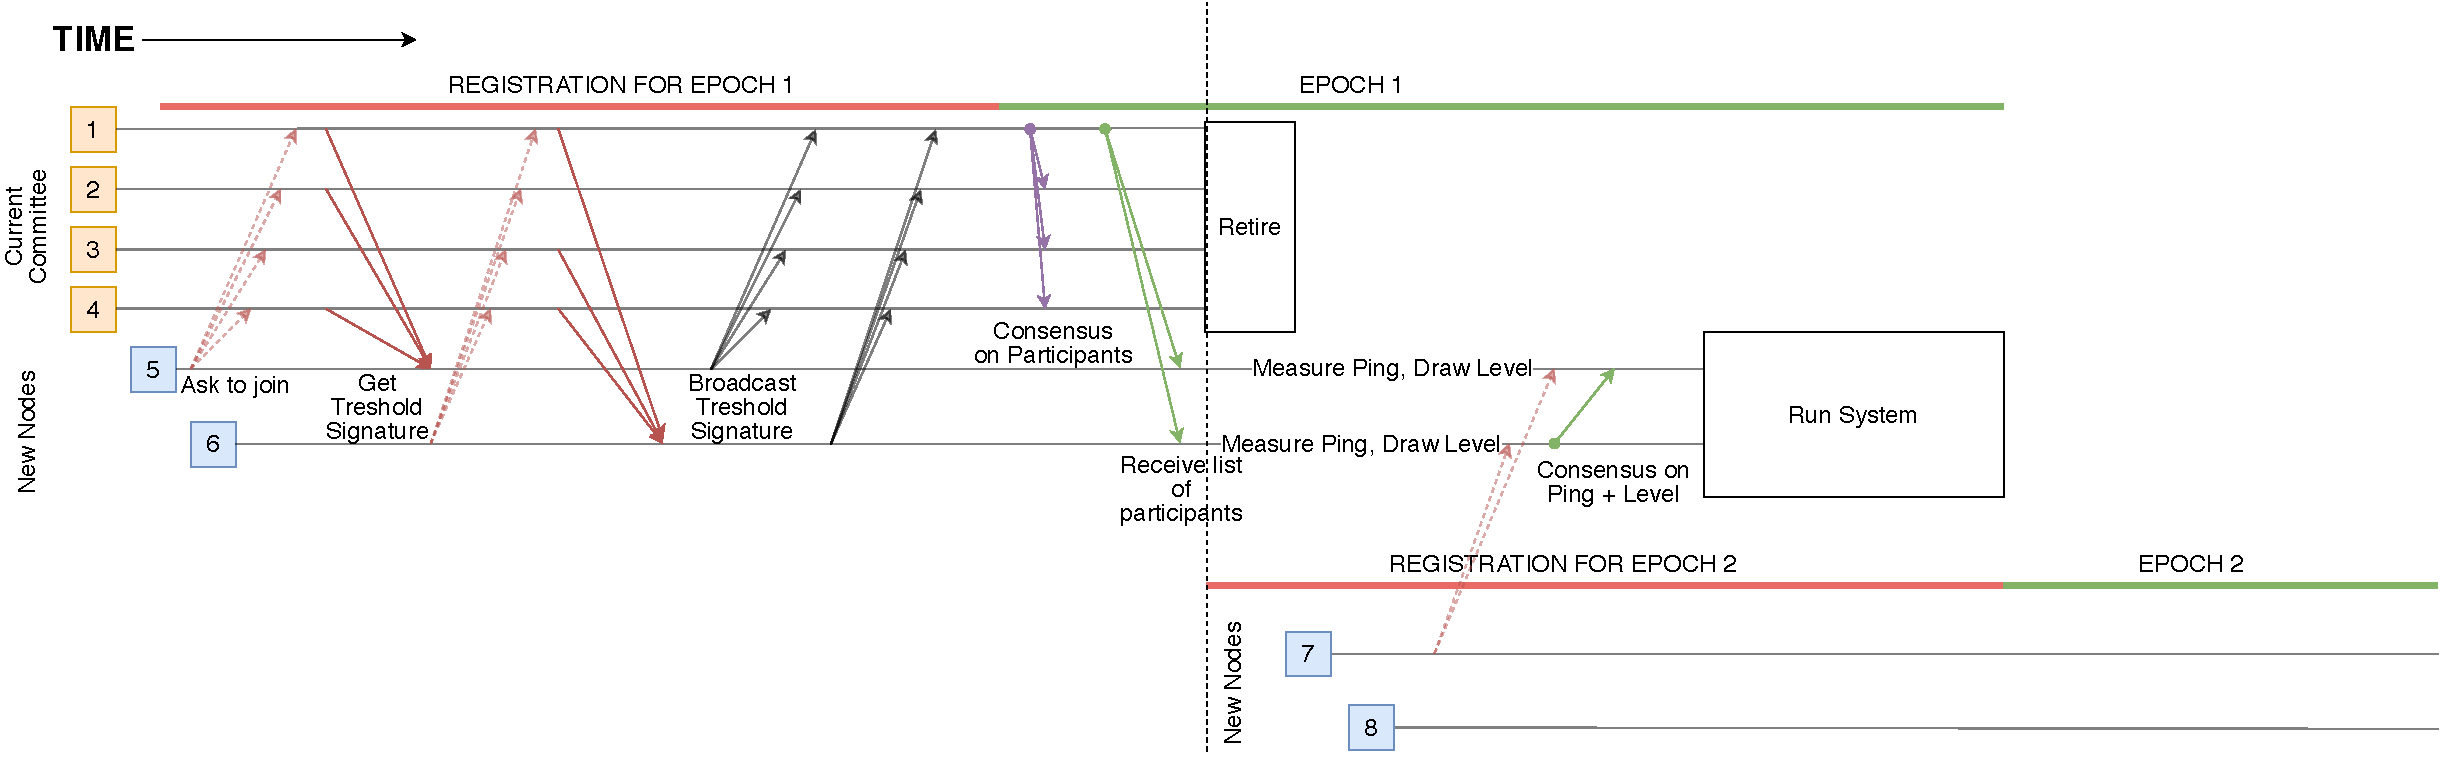
\includegraphics[width=700pt]{figures/Registrationprotocol}
\caption{Sketch of the Protocol. \color{red} TODO : SMALL CORRECTION \color{black}}
\label{fig:registrationprotocol}
\end{sidewaysfigure}

This section describes the membership protocol [FIG. \autoref{fig:registrationprotocol}].
The system will go through some cycles (called epoch) of two different phases :
the registration period and the live period. The first period is actually there
to manage the participants of one current epoch, and the “underlying system”
(for example a cruxified-blockchain) will be run during the live period. Assume
that each node has a synchronized wall-clock which gives the time of the
different periods.

The authority that will decide which node participates in the next epochs are
the participants of the current epoch, which will be called the admission
committee. Assume that a set of genesis participants, which will be the first
admission committee, exists.

\paragraph{Registration Period}
If a node wants to register for the next epoch, it has to send the following
information to the admission committee : a name, a public key, and an
endorsement (for example solution to a proof-of-work problem) and ask for a
threshold-signature. 

If the new node manages to get back a threshold-signature from the current
committee, it has to broadcast it again to the admission committee during the
same registration period. The current committee will then acknowledge that it
is a participant for the next epoch. The admission committee will aggregate the
threshold-signatures for all the participants for the next epoch. At the end of
the registration period, the admission committee will reach a consensus on the
new participants, by threshold-signing the list of the members.  

\paragraph{Live Period}
At the beginning of the live period, one member of the admission committee will
send the threshold-signed list of the participants to the current members. If
one of the participants did not receive the list, it can ask any member of the
admission committee to have it. After that propagation, the admission committee
can retire, and the member of the current epoch becomes the new admission
committee. Then members of the new epoch will compute ping-distances between
each other. Participants will as well draw a level from unpredictable,
bias-resistant public randomness source. They will then reach consensus on
those ping-distances and levels by threshold-signing them and rebroadcast them.
At this point each member of the new epoch will have the same view of the
system as they will know the participants, the pings distances between each one
of them and their levels. Therefore these participants will be capable of
running the system in a deterministic manner.

Following the election of the new admission committee at the beginning of the
live-epoch, the registration period for the next epoch can begin, as the
authority that will accept admission is running. Registration period and live
period can therefore be superposed [FIG. \autoref{fig:registrationprotocol}], which
permits to have a system running at every time. 

\subsection{Threshold-Signing Admission}
To get an admission a node that wants to join for the next system will use the
BlsCoSi protocol \cite{Boneh2018}. It will generate a tree with him as
the root and the admission committee as nodes in the tree. Each node of the
admission committee will have the choice of signing or rejecting the admission
query. The threshold will be set at the majority. So if a node manages to get a
majority of signatures then it will be accepted in the system, A node from the
admission committee is supposed to accept the query if it has not already seen
the node, and if the endorsement is convincing and was made with the public-key
associated. This ensures that a node cannot steal the endorsement of another
for registration.  

\subsection{Committee Consensus}
Committee consensus is used at two different times. First at the end of the
registration period. Consensus should be reached by the admission committee to agree on
the participants of the next epoch. A random member of the admission committee
is selected to run the consensus protocol. It will send the list of members
that it aggregated during the registration period. And try to get a threshold
signature on it from the other member of the admission committee. Members of
the admission committee are supposed to sign the list if they aggregated the
same list of members for the next epoch.

If one member does not manage to reach consensus, another can be selected to
run the consensus. A communication round can be added between two consensus
phases in order that every member of the admission committee broadcast its list
of members with valid proofs.

The same idea is used at the beginning of the live epoch to reach consensus on
the list of pings between every member of the system and on the levels on all
nodes in the system.
% TODO : think on what to do if the consensus is not manageable. 

\subsection{Public distributed source of randomness}
To draw the level to run the region creation algorithm, a distributed public
source of randomness will be used. This can be targeted by adversaries trying to
get a higher level and thus a higher place in the system. To be sure that this
source is not targeted, it is  based on the information created during the
consensus on the participants just before drawing the regions. 

\FloatBarrier
\section{Discussion}
\subsection{Advantages}
This simple version of the control plane is actually solving the problem of
churn and nodes movement in the system. A comparison will be made with a fixed
version only using CRUX for region management but without control plane. The
system begins with a fixed number of nodes and create regions based on CRUX,
then the system is replicated inside all regions. 

\subsubsection{Nodes insertion}
The version without control plane cannot add nodes to the system. Indeed a
fixed number of nodes is required to create the regions. With this control
plane, node insertion is possible at the beginning of every epoch
\autoref{fig:insertion-comparision}.

% TODO add image
\begin{figure}[!h] 
\centering
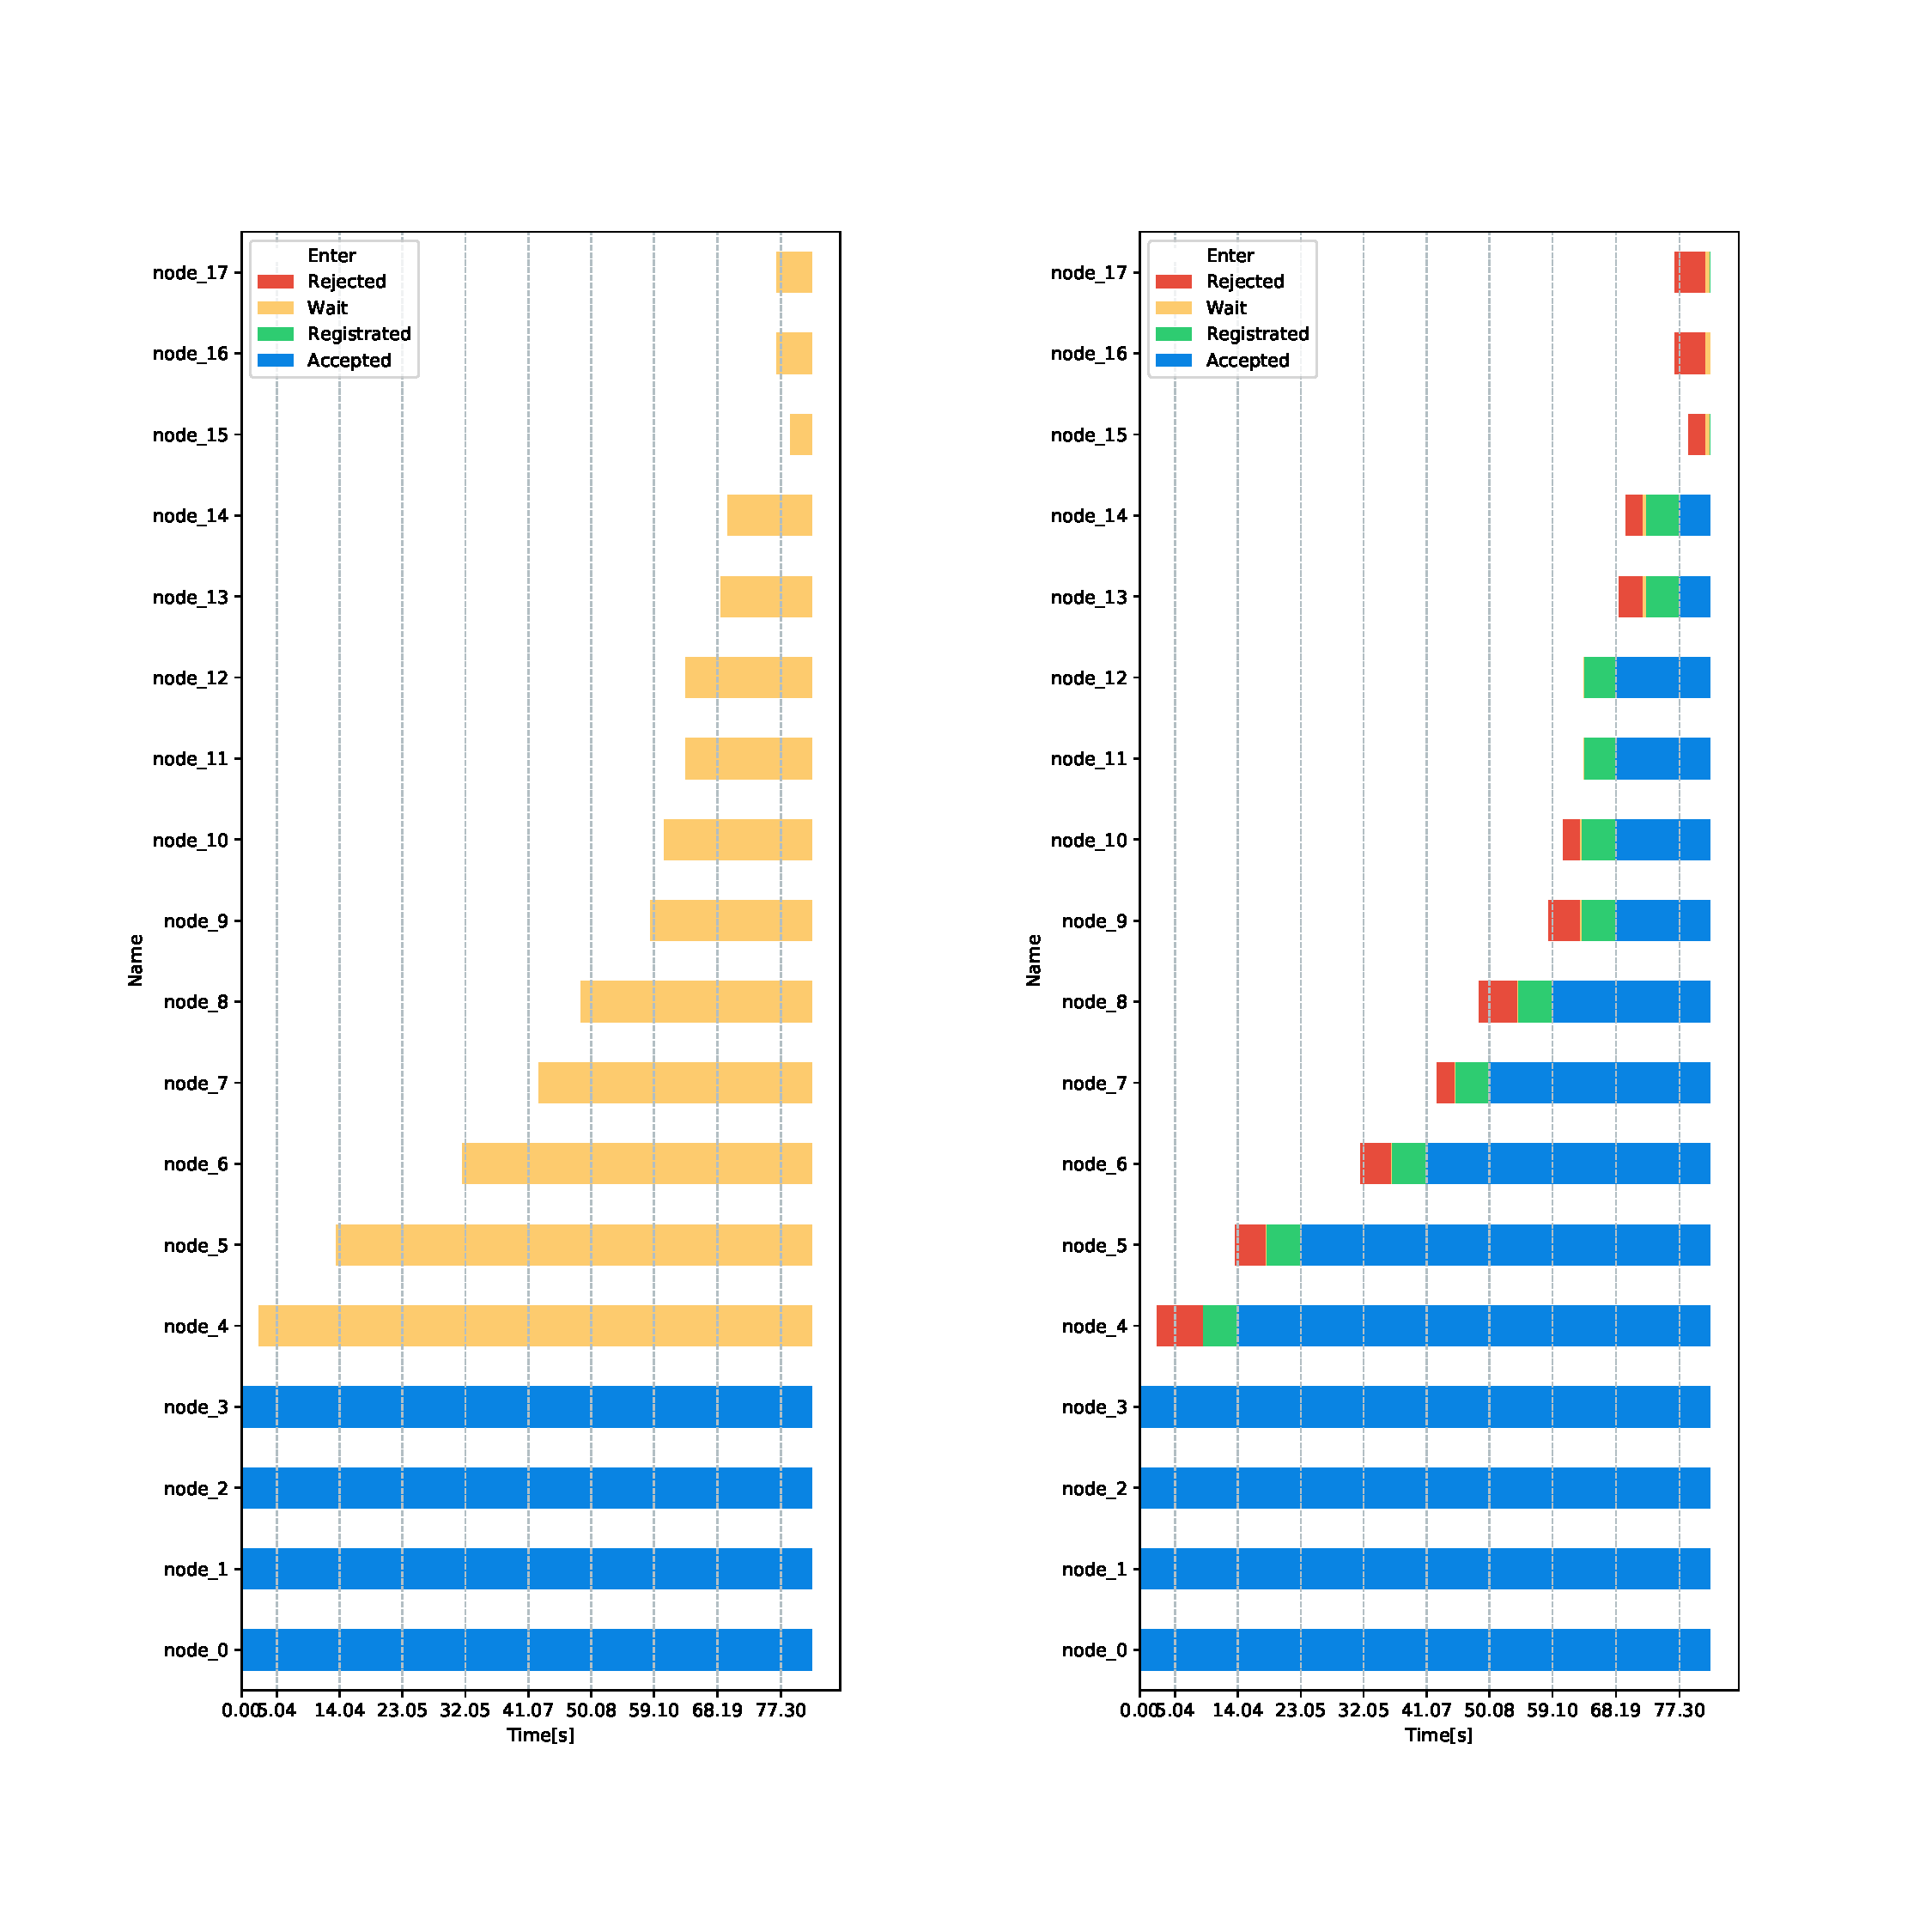
\includegraphics[width=450pt]{figures/JoinSubplots}
\caption{The simple control plane allow node to join the system. The left plot represents the case with a fixed control plane where node cannot join. The ticks are placed at the start of epochs. }
\label{fig:insertion-comparision}
\end{figure}

\subsubsection{Churn resistance}
Nodes can churn. If the system is not supposed to change, crashing nodes can still be
in the system. With this control plane, nodes that have crashed cannot
register for the next epoch and therefore are removed from the system \autoref{fig:churn-comparision}. 
% TODO add image 
\begin{figure}[!h] 
\centering
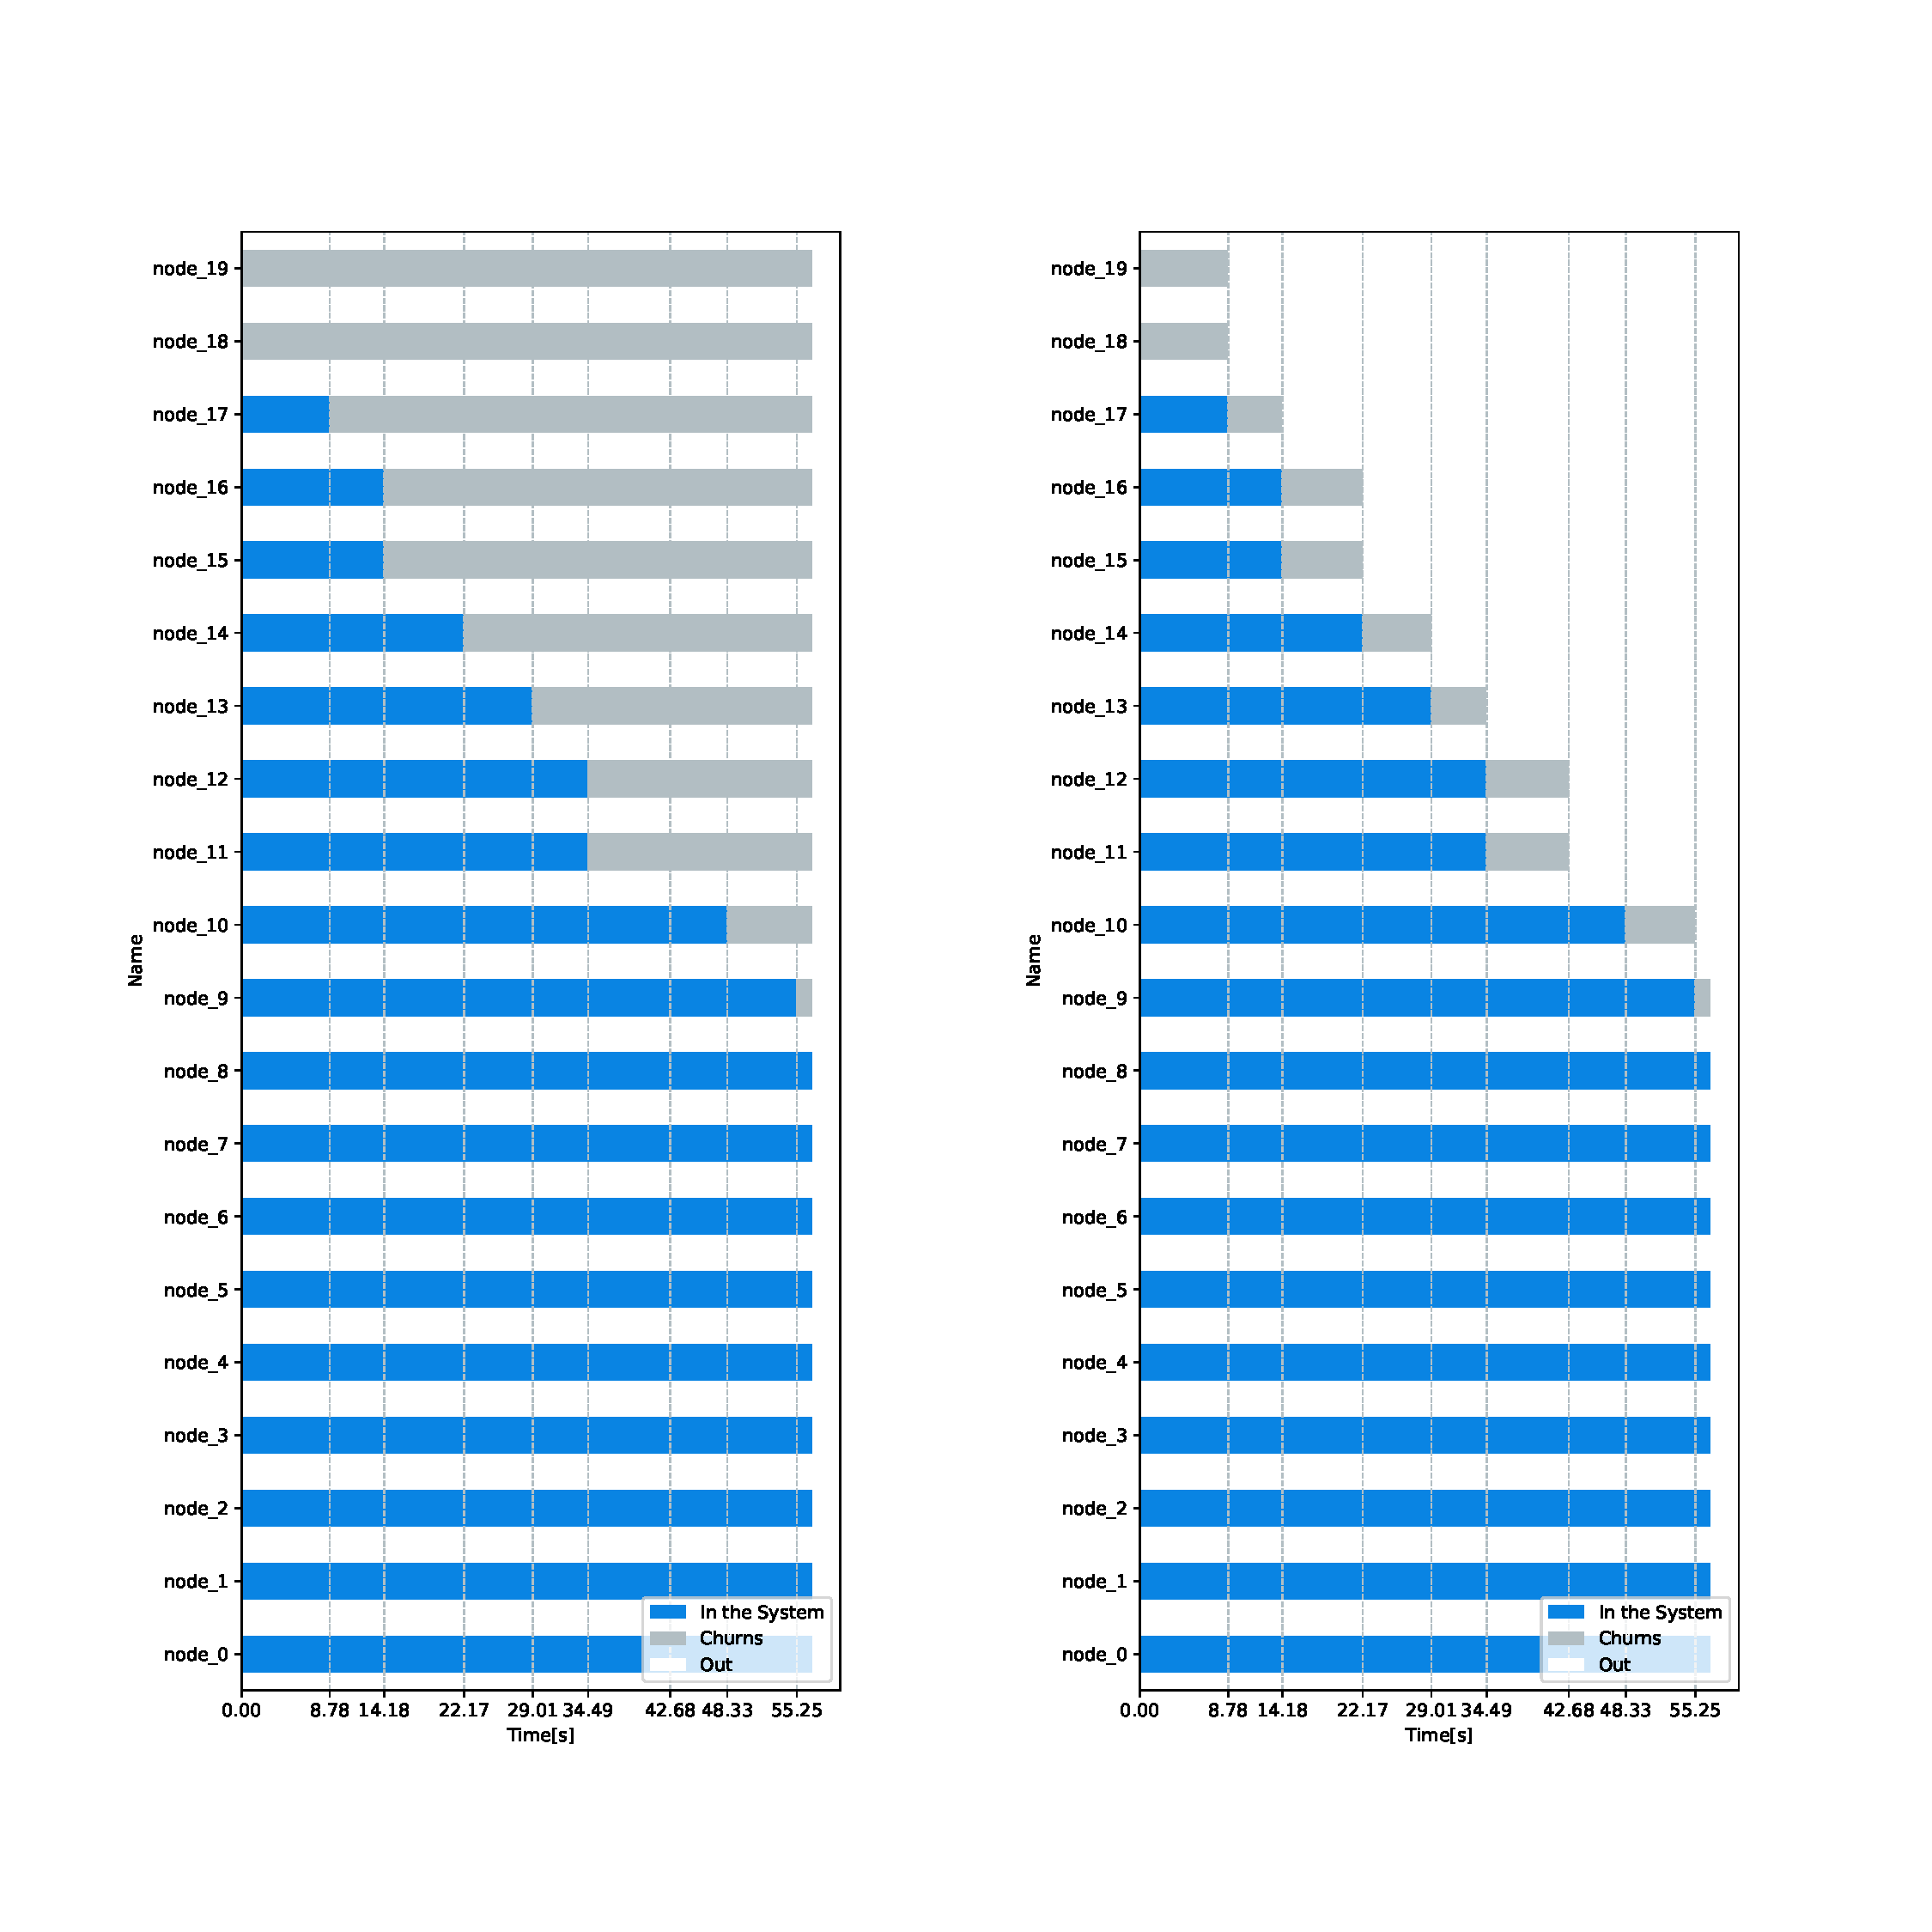
\includegraphics[width=450pt]{figures/ChurnSubplots}
\caption{The simple control plane remove nodes that have left the system. The left plot represents the case with a fixed control plane where node cannot leave. The ticks are placed at the start of epochs.}
\label{fig:churn-comparision}
\end{figure}

\subsubsection{Adaptation to Node Movements}
Nodes can move as well, if the regions are only drawn at the beginning of the
system. Then it's possible that after a while a lot of nodes have migrated from
where they were at the time that the regions were drawn. This might be a
problem, indeed, the purpose of the replication was to ensure that in case of a
partition, nodes participating in the same side of the partition should still
be able to work. If most of the nodes have moved, but are still participating
in the region of their first assignment, a partition could happen somewhere in
the system leading to failing regions that should be on the same side of the
partition. The control plane solves this problem as the region are redrawn at
each epoch taking account of the movement of the nodes. Increasing the
partition resistance, with the movement of nodes.

\subsection{Drawbacks}
This control plane is simple and reach its objective, but it requires a lot of
resources. Some of the drawbacks of this approach are listed below. 
These drawbacks are addressed in the section Improvements.  

\subsubsection{Control Plane is global}
If the system is replicated in all the regions, the control plane itself is
global. Meaning it could be subject to a partition. In this case the replicated
system would continue to work, but the control plane could only continue to
work on the side of the majority. This is not a major drawback as the main
purpose, the continuity of the underlying system is guaranteed.

\subsubsection{Epoch Transition Requires Resources}
Epoch transition requires a lot of resources, indeed first it needs a lot
communication for the consensus and the registration as every node that were
previously on the system should be contacted by every new node. If $N_i$ is
the number of participants at epoch $i$. Then registration for epoch $i+1$
requires $O(N_i * N_{i+1})$ messages. As every new node has to send a message
to every member of the previous committee. This can be really inefficient. 

Then when the registration is done, the protocol as it is will redraw most of
the regions as the algorithm for region creation is reused. This can be
inefficient as well, and it is then for the transition to happen, a copy of the
whole underlying system at epoch $i$ should be replicated in each new region of
epoch $i+1$.

%% TODO FIT
\begin{figure}[!h] 
\centering
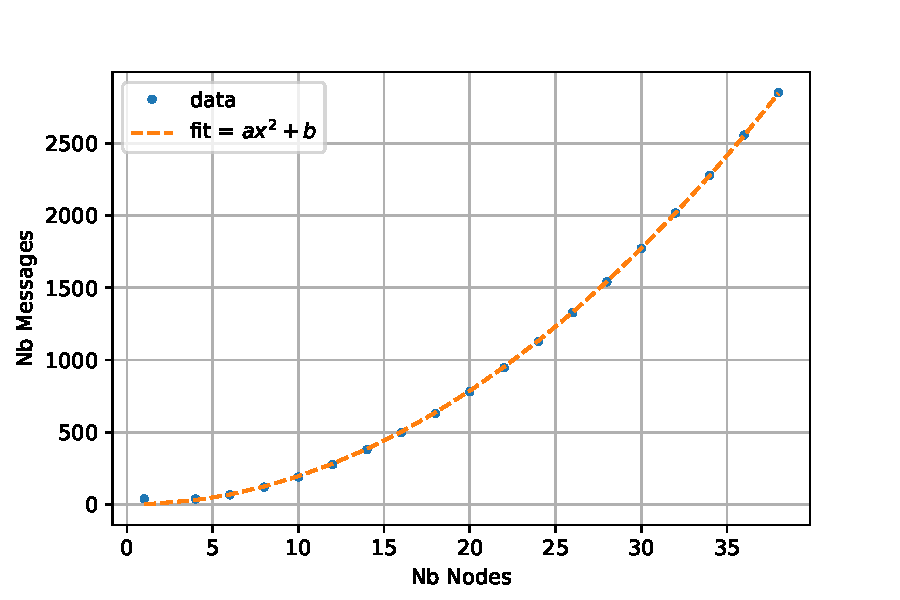
\includegraphics[width=350pt]{figures/messages-plot}
\caption{Growth of the number of messages for one epoch with the number of nodes. \color{red} TODO FIT \color{black}}
\label{fig:messages-plot}
\end{figure}

%% TODO FIT
\begin{figure}[!h] 
\centering
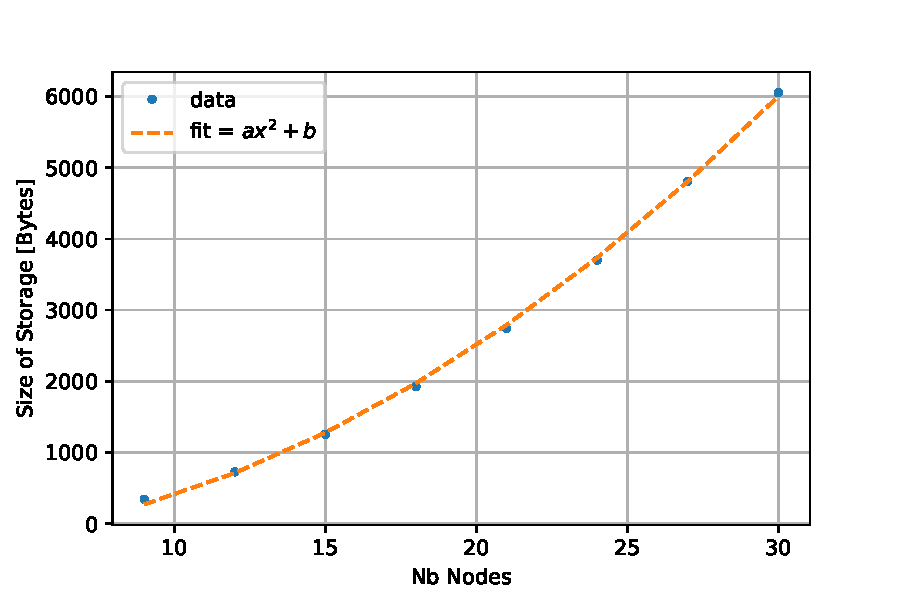
\includegraphics[width=350pt]{figures/storage-plot}
\caption{Growth of the number of storage for ping distances for one epoch with
    respect to the number of nodes. \color{red} TODO FIT \color{black} } \label{fig:storage-plot}
\end{figure}

 
\subsubsection{Omniscience of the Nodes}
Nodes are actually aware of a lot of information. By design they are aware of
the list of every other nodes in the system, their levels, the pings between
each pair of nodes in the system, all the region created and all the region
assignment. The nodes need to be aware of this information in order that
every node will run the algorithm for region creation and arrives to the same
regions. But this can be a lot of information to store.

\section{Security Analysis}

\subsection{Threat Model}
Attacks on the system can be made internally (from malicious nodes) or
externally by delaying the interaction between nodes or intercepting and
changing messages. We will give the precise portion of malicious nodes that
this protocol can handle. In this threat model, malicious nodes are regular
nodes that decides to act against the system. In particular, malicious nodes
have only access to a bounded computational power, and they cannot break the
cryptographic primitives. 

\subsection{Network Attacks} 
\subsubsection{Man-in-the-middle attacks} \label{MitM}
The messages exchanged during the protocol are listed in the following table  [\autoref{tab:messages-table}].

\begin{table}[]
\centering
\begin{tabular}{m{0.05\textwidth}m{0.3\textwidth}*{2}{>{\arraybackslash}m{0.2\textwidth}}}
\toprule
& Message                                                                                                       & Signature                                                       & Effects of a Sufficient Delay \\  \midrule
1 & Join request                                                                                               & Requesting node                                           & Request refused               \\ \hdashline[0.5pt/5pt]
2 &Threshold signature of the request                                                             & Threshold number of the current committee & Request refused               \\ \hdashline[0.5pt/5pt]
3 &Broadcasting of the Threshold signature                                                    & Threshold number of the current committee & Request refused               \\ \hdashline[0.5pt/5pt]
4 &Messages for the consensus on the participants,
list of the participants                                                                                       & Leader of the current committee                   & View Change                   \\ \hdashline[0.5pt/5pt]
5 &List of pings and levels                                                                               & Leader of the current committee                   & View Change \\ \bottomrule
\end{tabular}
\caption{List of the messages exchanged during the protocol. The signature of the message and the effects of a delay are given. }
\label{tab:messages-table}
\end{table}

As all the messages are signed, if a message is changed, it will be noticed by
the receiver. Which will discard the altered message, and ask again to the
sender.  Therefore the only effect of a Man-in-the-middle attack will be to
delete some of the messages, which is a sort of delay attacks. 

\subsubsection{Delay attacks}
This protocol is not really resistant against delay attacks. It assumes
wall-clock synchronicity between the nodes, which can cause some problems. The
effect of a delay of message are listed in [\autoref{tab:messages-table}]. During
the registration, if the messages are delayed until the start of the next
epoch, then it will lead to the refusal of the request, and the node have to
create a request again for the next epoch. If the messages of the leader of the
consensus for the participants of the pings and levels are deleted or delayed,
the other nodes will ask for a view change : asking the next node in the list
to start the consensus again.

\subsection{Malicious Nodes}
\subsubsection{Attack on Consensus}
If a malicious node is already in the committee, the only misbehavior that it
can do the period is to refuse to sign some messages. Re-sending wrong messages
are already treated in \autoref{MitM} as they are not possible to forge because
of the signature. Rsefusing to sign join requests can lead to a failing protocol
if the number of malicious nodes is bigger than the threshold required to get
the signature. As the signature procedure is done using BlsCoSi \cite{Boneh2018},
the registration process is subject to the same threat. BlsCoSi
\cite{Boneh2018} is an efficient way to implement The \textit{Practical
Byzantine Fault Tolerance} (PBFT) \cite{Castro1999} algorithm which guarantee
\textit{safety} and \textit{liveness} if the system as no more than $f$ faults
among $N = 3f+1$ nodes.Therefore it is required to have no more than $f$
malicious nodes. As the number of nodes in the system evolves
with time, it required not to have more than this fraction of malicious nodes
in the system at any epoch. If for one epoch, the number of malicious nodes is
bigger, then they can block all the consensus, leading to a failing system. 
If a malicious node is elected as a leader of the consensus on the list of
participants or on the nodes, it can decide not to start the consensus. After a
while, another node will be elected to run the consensus, which will eventually
succeed if the number of malicious nodes is low enough.

\subsubsection{Attack on levels} \label{sec:ControlePlane-Threat-Model}
At the beginning of one epoch, nodes compute their bunch and cluster based on
the pings and the levels that are drawn from a shared public source of randomness
which is renewed at each epoch. Nodes deploy region covering its cluster. Each
node will participates in regions along its bunch. This procedure however is
not based on the action of a nodes, but just on the fact that they exist at a
given place and a given level. What is meant by that is that every nodes have
the same view of the system. And if node $A$ have node $B$ in its bunch, then
node $A$ is supposed to participates in a region which is based on the position
of $B$ and spans the cluster of $B$, but $A$ already has all the informations
to know about this region using only the pings and levels. Therefore node $B$
cannot use a high level to perform action that will block the system. 

However, if a malicious attacker could take over the lottery process, it could
manages to group the high level in a side of the system. Leaving only the
level-zero. This could lead to some problem [APP. \autoref{app:levels-zero}].
Taking over the lottery process should not be possible by design.  Indeed, the
lottery is based on a public source of randomness that renewed at each epoch,
and revealed after the registration of the levels. Nodes can know the level of
other nodes, because they base the compute of their levels on the
threshold-signed list they received from the previous committee.  It is
important that the source is revealed after registration of the levels,
otherwise malicious nodes could try to influence the order of the list on which
the lottery process is based. 

%%%%%%%%%%%%%%%%%%%%
\chapter{Improvements} \label{chap:Improvements}
%%%%%%%%%%%%%%%%%%%%
This section proposes some improvements to the simple control plane approach. They
are supposed to address the drawbacks of the simple protocol, each improvement
will be illustrated in a Strawman model. Finally, an advanced
version of the control plane that uses a region creation algorithm based on
time/space graphs will be proposed. 

\section{Strawman 1 : Locarno Treaties} \label{Locarno}

\begin{figure}[!h] 
\centering
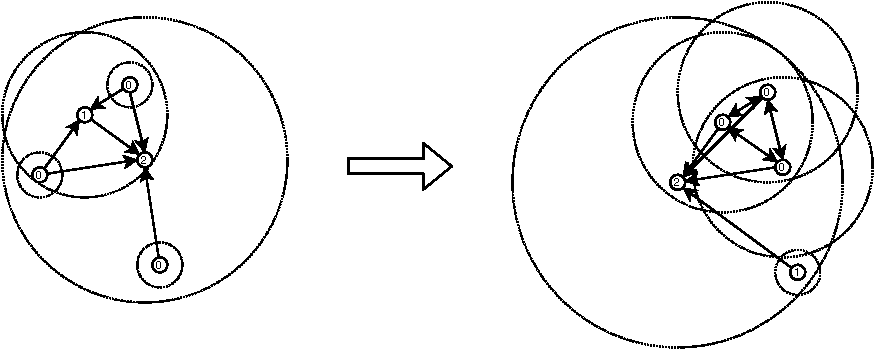
\includegraphics[width=300pt]{figures/LocarnoTreaties-Redrawing}
\caption{Redrawing the levels at each epoch can leads to very different version
    of the system. This is what is improved by the Locarno Treaties. Shrinking
    regions are depicted in red, growing regions in green and same region in
    black.} \label{fig:LocarnoTreaties-Redrawing}
\end{figure}

Following the First World War, it was decided that the borders of Germany
should remain fixed. The Locarno Treaties defined some of these borders. The
idea of this Strawman model is to do the same by limiting modifications of
regions from one epoch to the next. The idea is to use a deterministic set of
rules, based on the ping, the registrations and the map of the previous epoch
to draw the map of the current epoch using the less redrawing as possible.
Registration is still global and each node will have all the information about
the memberships of every node.Then from one epoch to another, the purpose of
the game is to keep as much regions as possible. The obvious idea to reach this
goal is to let the nodes keep their levels from one epoch to the next.  However
some small difference should be introduced in order to avoid some problems.
These are described in the next section.

\subsection{Rebalancing the levels} \label{rebalancing}
Conserving the levels is the way to go, but maintaining levels can lead to
unequilibred systems. Consider a system with 200 Nodes at epoch 1, with the
repartition given in \autoref{example-lottery}. If from epoch 1 to epoch 2,
100 level-0 nodes leave the system, the remaining system would contain 80
level-0 nodes instead of 90. 

Unbalanced systems can lead to some problems, the proof is given in the
appendix [\autoref{app:unbalanced-levels}]. The lottery process presented in
\autoref{sec:common-tools}, is a bit changed in this part to allow the
adaptation of the levels. The total number of participants $N$ in the system is
known after the registration, and as the probability $P$ is given, it is
straightforward to compute the expected number of nodes that one should have at
every level as it mentioned in \autoref{example-lottery}. 

Instead of drawing directly the levels from a randomness source, nodes will
draw a random number from this source between 0 and 1
[\autoref{fig:sketch-new-levels}].  All nodes can deduce what number the others
will draw deterministically from the registration list.  The highest level will
go to the node which has drawn the highest random number.  And levels are given
according to the drawing in a descending order.  Each node that stays in the
system will keep its random number from when it joined the system, new nodes
gets new random numbers. 

\begin{figure}[!h] 
\centering
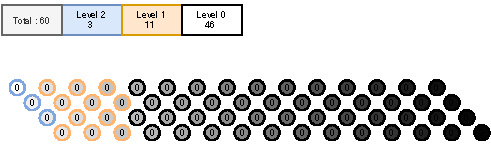
\includegraphics[width=400pt]{figures/Lottery-Locarno}
\caption{Sketch of the new method for drawing the levels. The fill represents the number that was drawn from 0 (black) to 1 (white).}
\label{fig:sketch-new-levels}
\end{figure}


\subsection{Motivation for keeping the levels}
This section describes the reasons for keeping the levels. In order to
understand what are the effects on the global system it is useful to look in
detail at what are the consequences of the movement of a given node have on a
given fixed node. Then some precise examples of evolution of the system are
treated as well. 

\subsubsection{Effects for a fixed node} 
The point of view of one node that stays fixed in the system is taken, the goal
is that node can keep most of its region assignment.  Other nodes might
join, leave or move and this can lead either to change in its cluster of in its
bunch. But additional effects can come from the level rebalancing. 

\paragraph{Nodes Leaving the Cluster} 
This can shrink the cluster. As the regions created by a given node stops when
the radius covers the whole cluster, this might lead to the deletion of some
regions. This does not change the
region assignment and the nodes can still keep the replicated system of the
previous epoch running. But additional effects can come from the level rebalancing. 

\paragraph{Nodes Joining the Cluster} 
On the contrary, if nodes join the cluster, this might lead to the creation of
additional region to cover these extra nodes. The node will then replicate its
system to the newly created regions. But most of the regions are kept the same.

\paragraph{Nodes Leaving the Bunch} 
Nodes participate to all the region in their bunch, eventually they will
participate to a region that spans the whole system. If a node left the system
in the bunch,  this leads to a region centered around a point that is not in
the system anymore, this assignment might be forgotten. 

From the point of view of a node, if another node leaves its bunch, it can have
as effect to add other nodes in its bunch, leading to more region assignment.
And in some cases, to more nodes in its cluster, leading to region growth. 

\begin{figure}[!h] 
\centering
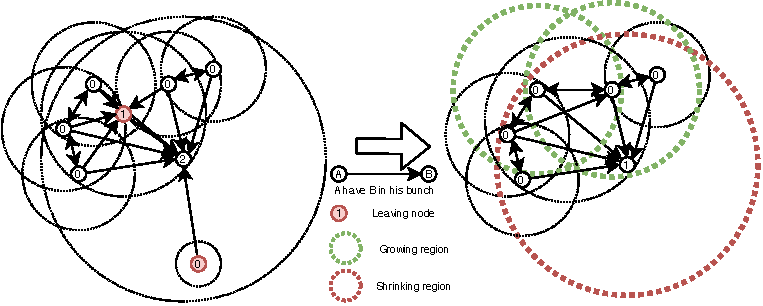
\includegraphics[width=300pt]{figures/LocarnoTreaties-Leaving-cluster}
\caption{A leaving node is changing assignments of other
    nodes but keep the same regions. Shrinking regions are depicted in red,
    growing regions in green and same region in black. }
\label{fig:LocarnoTreaties-Leaving-cluster}
\end{figure}

\paragraph{Nodes joining the bunch} 
If nodes are joining in a bunch, this leads to additional region assignment. 

\subsubsection{Rules for other nodes}
Moving nodes or joining nodes are different, they are joining a new region, the
question is how to integrate them in the system while keeping the system
balanced. 

\paragraph{High level node moving}
Assume that going from Epoch $i$ to $i+1$, one of a relatively high-level node
as gone from one place to the other end of the system. As nodes can keep their
level, it will change some of the assignments, but most of the regions will be
maintained. 

\begin{figure}[!h] 
\centering
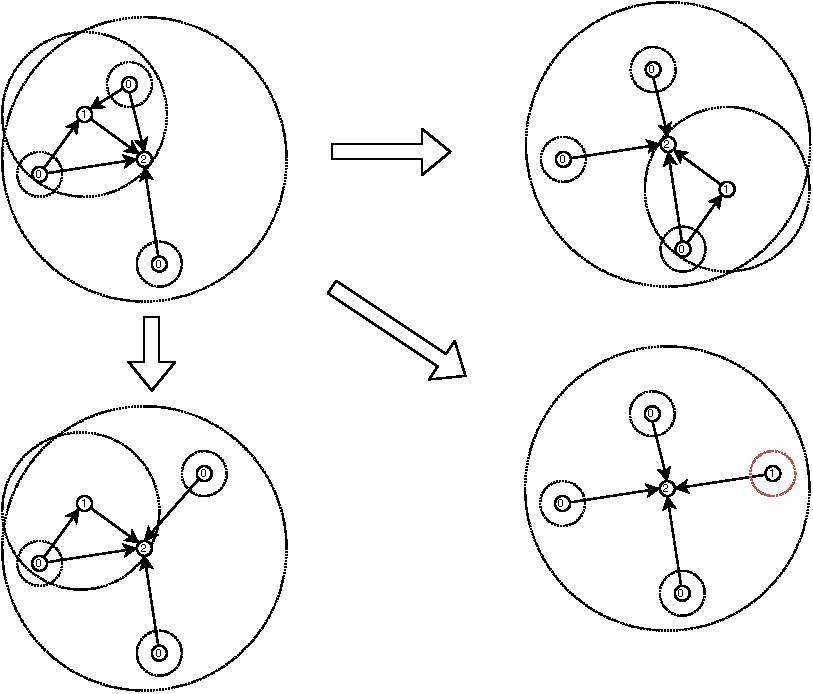
\includegraphics[width=300pt]{figures/LocarnoTreaties-Moving}
\caption{A moving high-level node keeping its levels is changing assignments of other
    nodes but keep the same regions. Shrinking regions are depicted in red,
    growing regions in green and same region in black. }
\label{fig:LocarnoTreaties-Moving}
\end{figure}

This seems to indicate that movement should not be a problem. There is a
slight difference between that situation and redrawing the levels at each
epoch. As each node can keep its copy of the underlying system working in its
region. If the levels are redrawn, communication might be needed to transfer
knowledge from one region to another. This communication overhead is reduced in
that situation. 

\paragraph{Levels of joining nodes}
One can think that the levels of joining node might have a big influence on the
system, this part try to illustrate what might happen.  The joining nodes can
lead to the growth of one region or the creation
of regions. The precise rules for that are listed below. 

\begin{figure}[!h] 
\centering
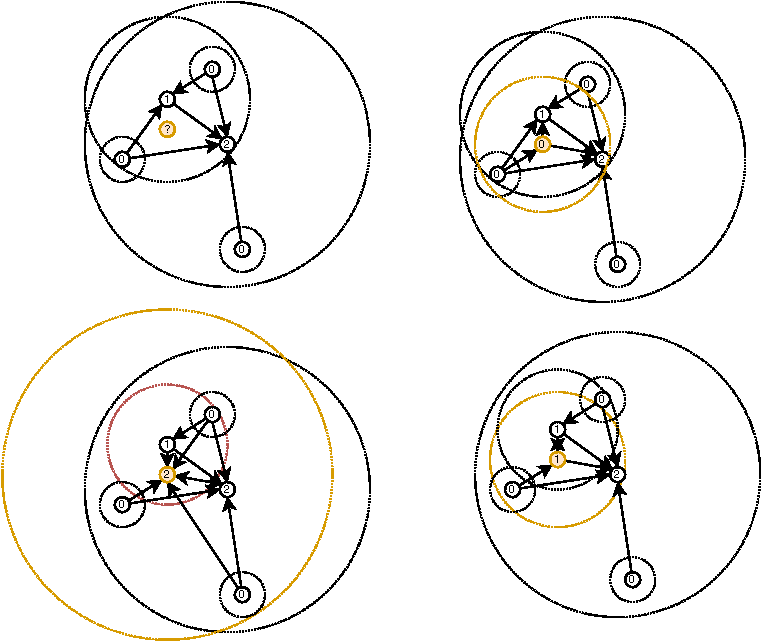
\includegraphics[width=300pt]{figures/LocarnoTreaties-Insertion-close}
\caption{Keeping the same level leads to smaller changes when a node enter the
    system. Shrinking regions are depicted in red, growing regions in green and
    same region in black.} \label{fig:LocarnoTreaties-Insertion-close}
\end{figure}

\begin{figure}[!h] 
\centering
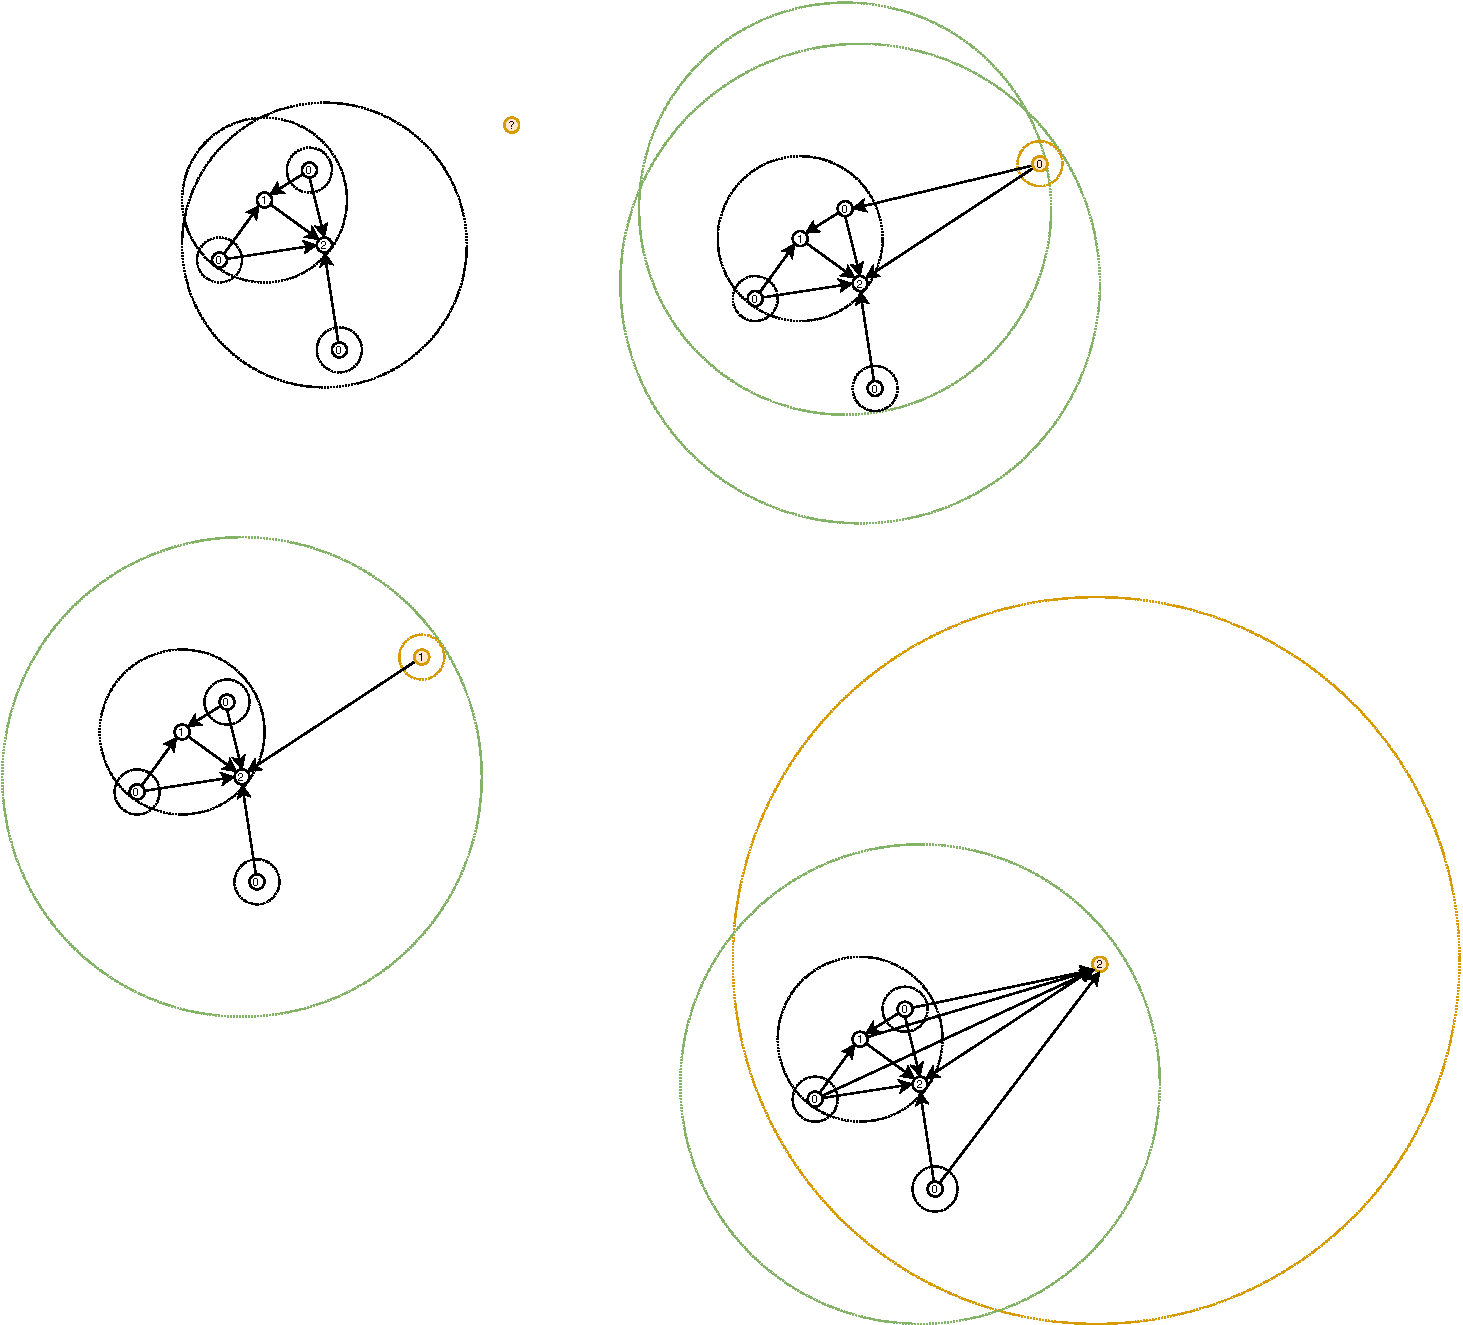
\includegraphics[width=300pt]{figures/LocarnoTreaties-Insertion-far}
\caption{Keeping the same level leads to smaller changes when a node enter the
    system. Shrinking regions are depicted in red, growing regions in green and
    same region in black.} \label{fig:LocarnoTreaties-Insertion-far}
\end{figure}

\subsection{Protocol}
The protocol is mostly the same as the simple control plane protocol [FIG.
\autoref{fig:registrationprotocol}]. The main difference is the level assignment
which follows the new algorithm described in \autoref{rebalancing}. 

\subsection{Threat Model}

The new lottery process can be targeted from attackers. But as it is equivalent
to the other one, attacks that are valid for one system are valid for this one.
But this will ensure to have the proper number of levels in the system in each
epoch.

If one node is not happy with its level assignment, it can leave the system a
re-enter later, hoping to get a better level. This attack works against the two
algorithms, but this attack does not create too
bad consequences, as it is presented in \autoref{sec:ControlePlane-Threat-Model}.

Another attack could be that malicious nodes exit and re-enter the system at
each epoch until they manage to get a good number from the lottery. Then when
it manages to get good level, they collectively move to one side of the system
leaving good nodes all at level-0 in the middle of the system. This will create
a slight overhead for the good nodes as the region’s assignment increase for
the level-0 nodes. But this attack seems to cost a lot of resources and
coordination for the attacker to generate a small overhead on the size of the
participants.

Some defense mechanisms can be set up to ensure that levels are geographically
distributed over the whole system, they are described in more details in
\autoref{chap:Possible Improvements}.

\subsubsection{Quantifying the effect of Locarno Treaties}
The goal of the new protocol is to keep most regions and region assignment
following the evolution of the system. 

A concrete comparison is made. The system starts with a fixed number of nodes
and evolves with nodes moving, leaving and entering the system. A metric is
chosen to evaluate the difference between the system from one epoch to the
next. The metric is defined as the following :  the list of participants in the
system is taken sorted by name. Then for each node, their bunch and cluster
will be compared. Each difference will be counted, if a new node enter the
system, their bunch and cluster count as a difference. Same if a node leaves
the system. The idea is that with this new protocol, the difference should be
reduced. 

The results of the experiment can be seen in [FIG. \autoref{fig:LocarnoTreaties-differences}]. Maps of
the system is given in the appendix [APP. \autoref{app:LocarnoTreaties-data}].

\begin{figure}[!h] 
\centering
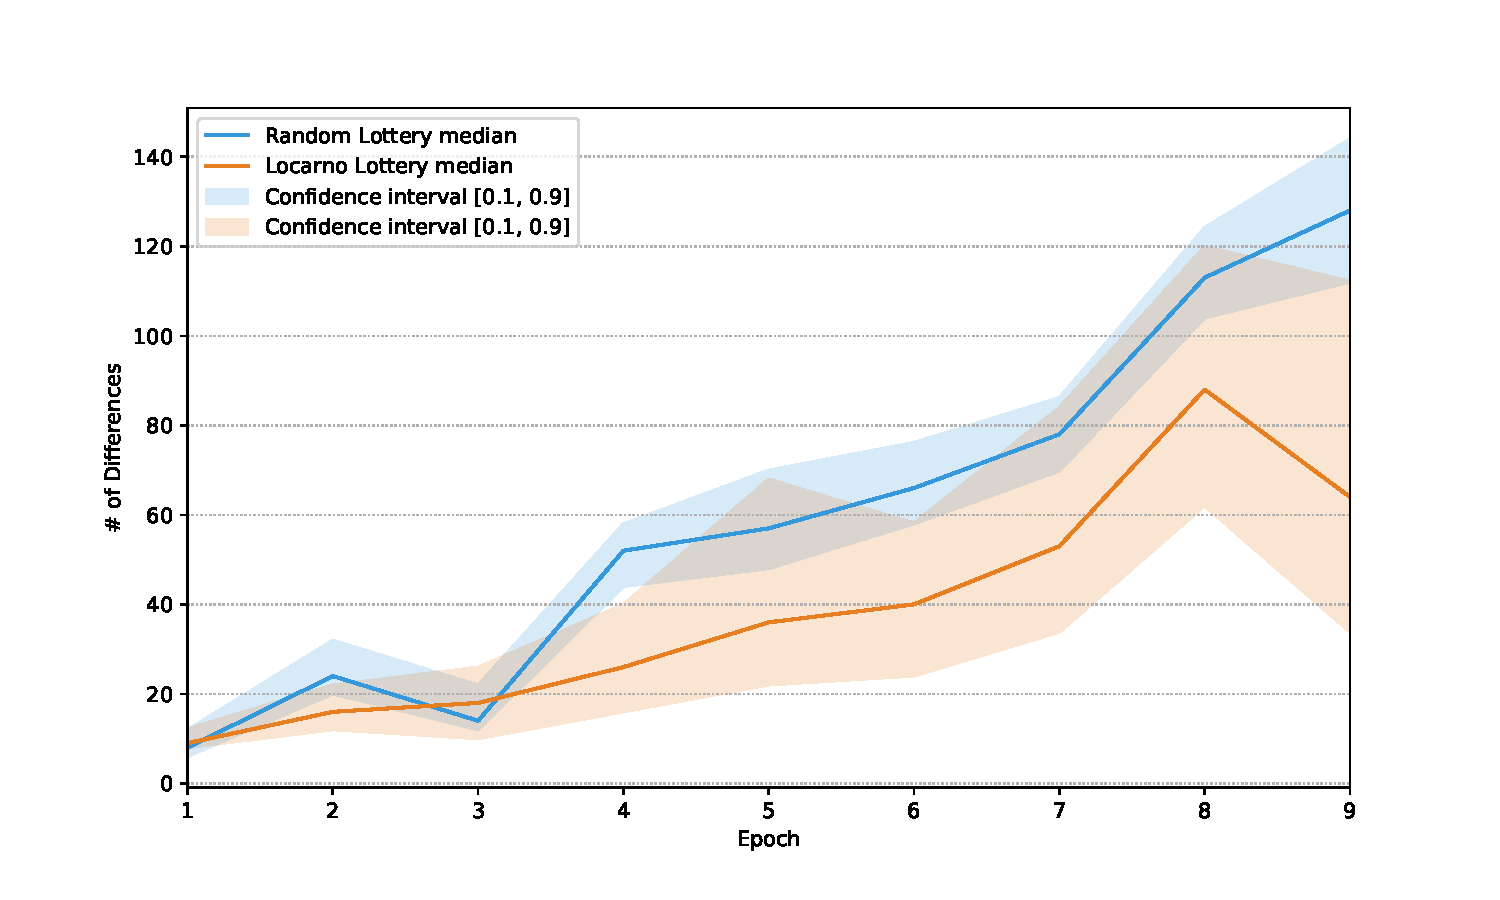
\includegraphics[width=300pt]{figures/LocarnoTreaties-differences}
\caption{Graph of number of differences between maps from one epoch to the next using the random levels or the one defined in Locarno Treaties } \label{fig:LocarnoTreaties-differences}
\end{figure}

\section{Strawman 2 : Fog of the War}

Each node of the system will have a different view of the world at a given time
depending on its place in the system and its interactions. Again the idea is
that one node should be aware of only the information it needs to perform its
actions. A correspondence can be made with the fog of war in some traditional real-time
strategy video game, where each player will have its own view of the system,
based on where it is now (light), where it was in the past but
cannot see now (fog) and what it has not already seen (dark).
Each player view will evolve through space and time accordingly. In the context
of the game, the advantage of this view is that it hides the adversarial
strategy. In the context of our system, this view will hide most of the
information that is not relevant to one node but allow it to perform its
operation without the storage and/or communication overhead. 

The design of this Strawman will be the following. Each node declares a
position during the registration, and other nodes computes their bunch and
cluster according to this declared position. Each node will therefore be able
to compute their bunch and cluster based on these declared position. To ensure
the correctness of the system a random committee of checkers are elected after
the registration process. These checkers will perform some tests (pinging other
nodes of one region) and publish the results. 

\begin{figure}[!h] 
\centering
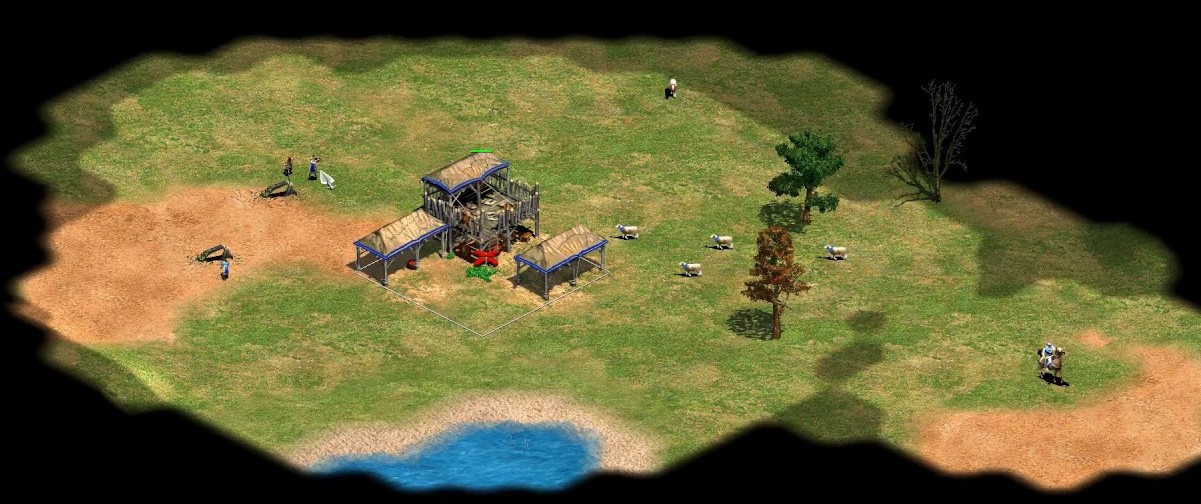
\includegraphics[width=400pt]{figures/fog_of_war}
\caption{Fog of war representation in a classic real-time strategy video game. }
\label{fig:registrationprotocol}
\end{figure}

\subsection{Purpose : Reducing the need of the Locality Component}
The protocol presented in the Simple Control Plane protocol and in the Locarno
Treaties still need a consensus on the pings between all nodes in the system.
This can be cumbersome as the number of nodes increases in the system this
quantity increases in $O(N^2)$, where $N$ is the number of node. Consensus
might become too costly for that reason.

The idea is to change that consensus with a declared position and a random
committee of checkers. The question is still : how to choose the committee ? If
sampled randomly the chances are big that the selected nodes will be far away
from each other, and above a certain threshold, the correlation between pings
and distances are not satisfactory. Therefore the committee of checkers can be
selected to be the $n$ closest nodes based on the declared distances. And $n$
can be adapted to increase if one node does not pass the checks. 

If a node does not pass, the checks it either means that this node is faulty or
that the number of checkers is constituted of a majority of malicious nodes.
One can solve the second problem by increasing the number of checkers $n$, and
progressively a majority of honest nodes should have checked the node. It the
ping still does not correspond to what the node declared then one might assume
that the node itself is faulty. 

\subsection{Protocol}
The protocol is mostly the same as the simple control plane protocol
[\autoref{fig:registrationprotocol}]. The only difference is the consensus on
the pings which are now replaced by a declared distance, which is announced
before the level assignment and a round of checks and announce of the checks. 

\subsection{Threat Model}
Another question can be, what are we supposed to do with a node that are not
passing the tests ? First it is important to notice that it won't actually
change the view that all nodes will have of the system, as nodes use the
declared distance to compute their bunch and cluster. But one node could use
that system to keep its level and virtually go to a strategic place where it can have
more influence. This is what one may want to avoid. 

There are three approaches to this problem, the first is to exclude the node
from the system, but it might lead to the redrawing of a certain number of
regions, and it might lead to attacks. Another strategy could be to define the
position of the faulty node with an approximation based on the ping. If we have
the position of the other nodes and we have to fix the location of the unknown
faulty node one might do that by computing the intersection between the circles
based on the pings. This triangulation strategy [\autoref{fig:triangulation_strategy}] can block one faulty node to
reach a desired position. 

\begin{figure}[!h] 
\centering
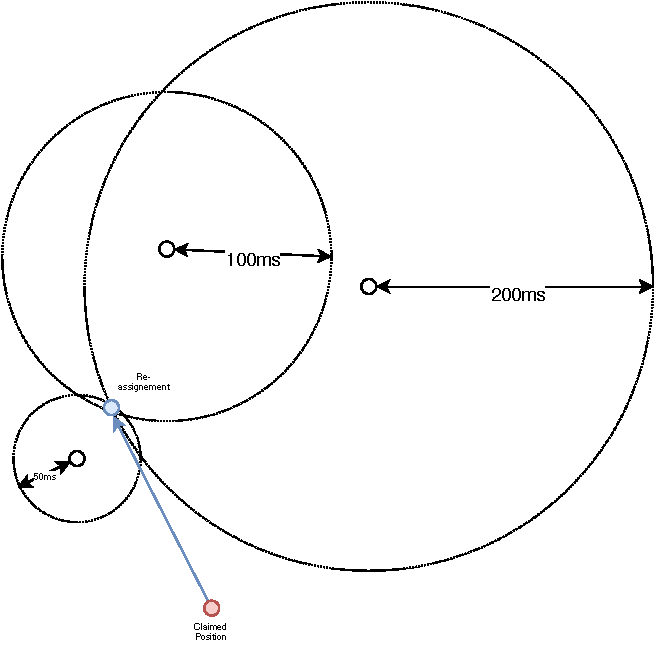
\includegraphics[width=300pt]{figures/triangulation_strategy}
\caption{Triangulation can be used to reassign the position of a faulty node.  }
\label{fig:triangulation_strategy}
\end{figure}

As nodes can announce a position and that is checked in priority by close
nodes, with this protocol if there is a sufficient number of malicious nodes,
they can declare that they all live in a close region and valid each other.
There is no simple solution to this problem, but that fact has no consequence
on the system so it seems to be an acceptable weakness.

\section{Introducing the Space/Time Interaction distance}
One of the principal reasons to split the system based on the locality is
because of most regular transactions between people are local, therefore one
wants to ensure that in case of a global partition, the local transactions can
still be processed flawlessly. Following this hypothesis, one can try to use
this structure to update the system. As there should be more interaction in
local regions. Most interactions can be processed locally. By using locality
the really goal is to maintain the interactions between the nodes. In that
case, the metric of distance is used to get an insight of the interactions. And
this is a reasonable approximation, but it might be worth it to investigate
directly what this interactions means. 

\subsection{Interactions as a distance on Space/Time Graphs}

If one wants to leverage the locality of interactions to build regions, it
might be worth it to investigate the following case.  Imagine that some nodes
$A$ and $B$ interacts often, but they are not part of the same small local
region.  By design there is a bigger region in which they interact, and each of
these interactions should pass by this bigger region. One property that might
be useful is that these frequent interactions should have an impact on the
system leading to the inclusion of one node in a "regional" region. If the
metric that defines distance is changed from kilometers to "interactions". One
should be able to redraw the whole system based on that, and to apply Crux to
solves the system. Now how to actually define this metric ? Let's try with the
following definition of distance : \begin{equation} \label{definition-distance}
    d(A,B) = \frac{1}{ \mathrm{\#\ messages\ between\ A\ and\ B\ per\ unit\ of\ time} } 
\end{equation}

\begin{itemize}
\item $d(A,B) = 0  \Leftrightarrow A = B$
\item $d(A,B) \geq 0$
\item $d(A,B) = d(B,A)$
\item \color{red} $d(A, C) \leq d(A,B) + d(B,C)$ \color{black}
\end{itemize}
\color{red} TODO cite metric space \color{black}

Interestingly the interaction metric follow this property. Indeed for the
first, we define that the number of messages that one node send to itself is
infinite. Second the number of messages is positive meaning that the distance
will always be positive. Third the interactions are counted as symmetric (if
$A$ is sending a message to $B$ we count that as an interaction between $A$ and
$B$). Actually the triangle inequality is not respected and that is a problem
indeed one should notice that if $A$ is close to $B$ and $B$ to $C$ but it is
possible that $A$ and $C$ never interacts therefore are "far from each other". 

\paragraph{Example :  CFF Distance}
A parallel can be made with the CFF distance. Indeed in some case it is much
faster to take a train from $A$ to $B$ and then to take a train from $B$ to $C$
than taking a bus from $A$ to $C$ [\autoref{fig:CFF-map}][\autoref{fig:CFF-NewDistances}] . 

\begin{figure}[!h] 
\centering
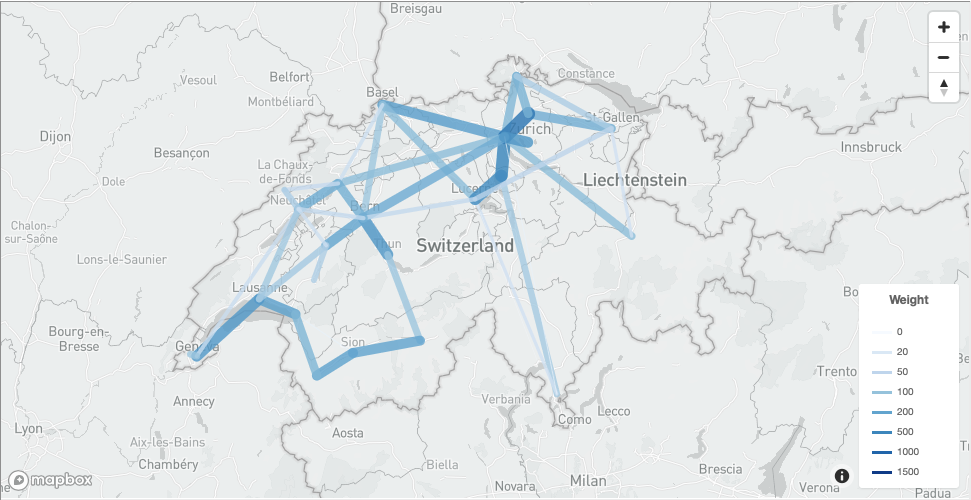
\includegraphics[width=450pt]{figures/CFF-map}
\caption{Map of the train network in Switzerland, line width is proportional to the number of connection per day.}
\label{fig:CFF-map}
\end{figure}

\begin{figure}[!h] 
\centering
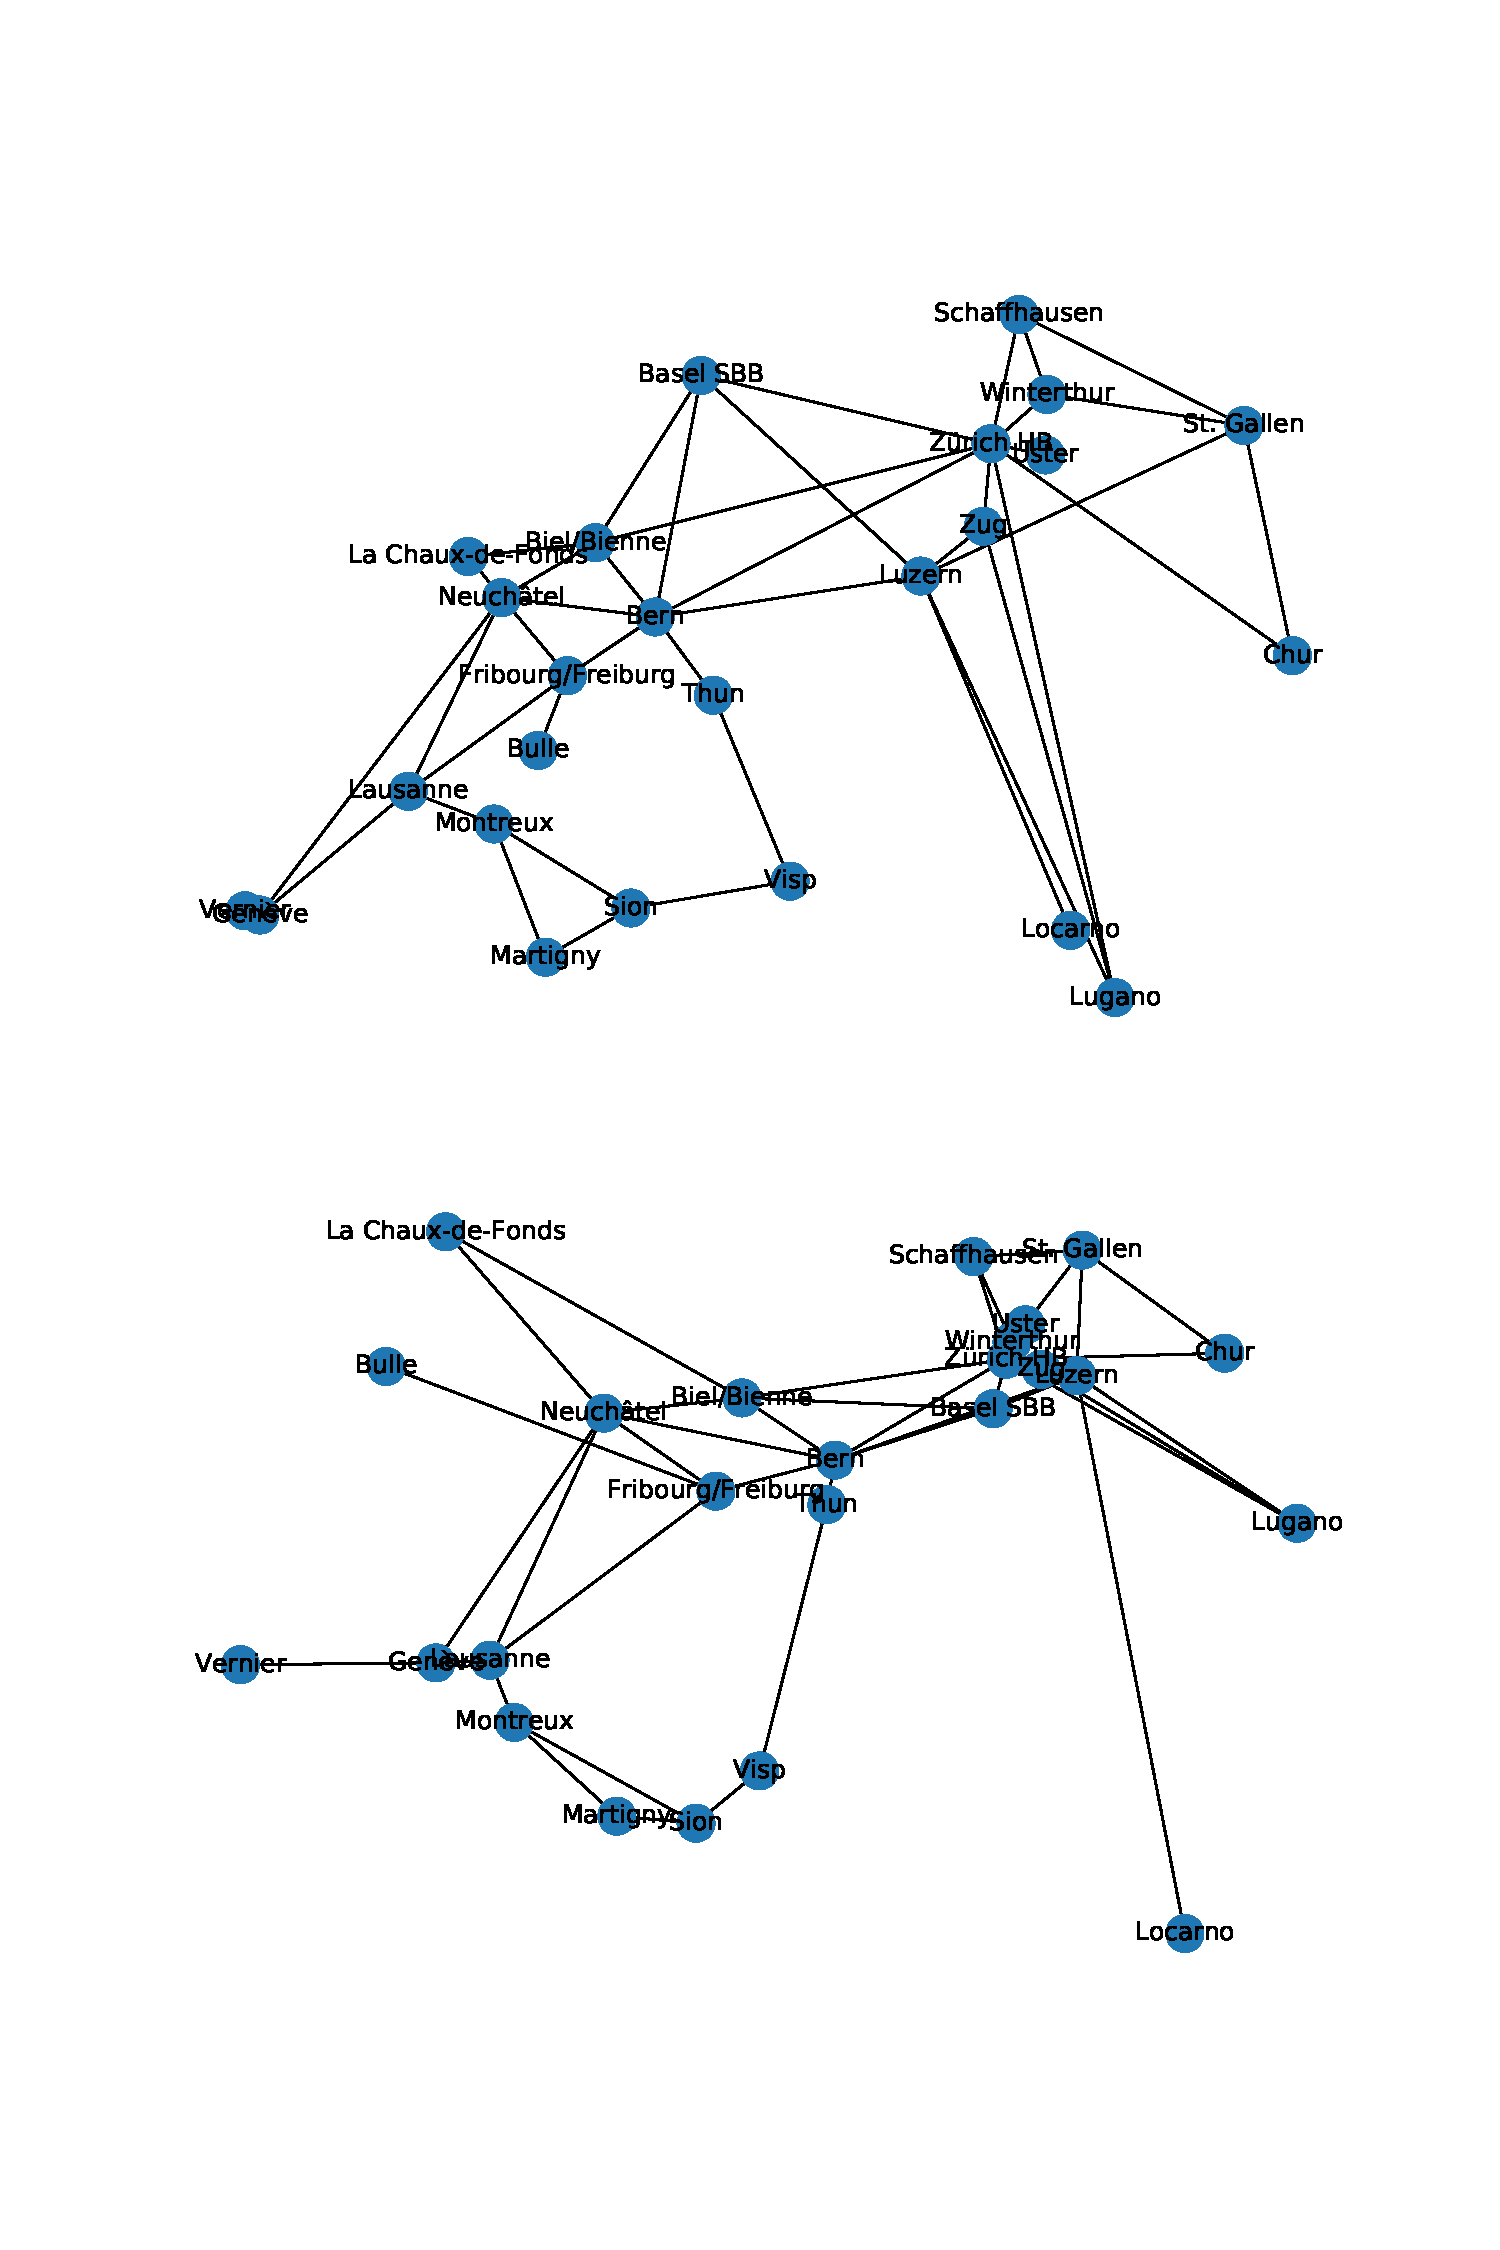
\includegraphics[width=350pt]{figures/CFF-NewDistances}
\caption{The train network is drawn again, using the regular distance first. In the second time the graph is displayed using the interaction distance as force in a force-directed graph. Ensuring that nodes that are close with regard to the interaction distance are close on the graph.}
\label{fig:CFF-NewDistances}
\end{figure}


\subsection{Finding Meaning}
In order to understand better what means this metric, the standard case is
considered. We want to understand what is mean to move with that new metric as
well as joining and leaving the system. 

\paragraph{Movements for Nodes With Interaction Distance}
It is easier to understand what it means to move in that space by looking to
the relative distance between nodes. Imagine that node $A$ get closer to node
$B$ but away from $C$ in that space. That means that the interactions between
$A$ and $B$ increases and on the contrary that the interaction between $A$ and
$C$ decreases.

\paragraph{Joining nodes with Interaction distance}
If a node joins the system and start to interact with others, this can be
viewed as a node coming from an infinite distance and getting closer to other
nodes.

\paragraph{Churning nodes with Interaction distance}
If a node churn and stop answering the other, this can be interpreted as a
movement in the interaction space. It equivalent at if the churning nodes moved
to infinity.  

\paragraph{"Regions" With Interaction Distance} \label{par:section-example}
The concept of the region is harder to conceive with that new notion of
distance. It might be useful to use the parallel with the CFF, let's imagine a
node at EPFL and try to conceptualize to what might correspond the equivalent
of "local", "regional" and "global regions". The "local" region might be
depicted with what places can be reached within 15 min of public
transportation. This will cover the metro line to Lausanne and some bus stops.
At the regional level, it might be what places are reachable within 1 hour of
public transportation. Global level still covers all the nodes.

\subsection{Justification to replace the locality}
Changing the distance from the regular one to interactions might have some
implication on the property that we want to keep in the system. 

\paragraph{Partition Resistance}
For partition resistance actually even more than preserving working region
composed of geographically close nodes it might be more interesting to preserve
the set of nodes that have a lot of interactions. As this might be the nodes
that are doing the most operations of the system. This justifies the use of
this new distance.

\paragraph{Region Validation for Transaction}
One problem that Nyle wanted to solve was region validation, to allow a fast
processing of transaction. This is still possible in that case. However the
region does not correspond to the same anymore. But they would correspond to
the example depicted in \autoref{par:section-example}. This might be acceptable
for a client. 

\subsection{Protocol}
The protocol is the same as the one described in Locarno Treaties
\autoref{Locarno}. The only difference is that the distance is changed by the
new metric \autoref{definition-distance}. The computation of the number of
messages is done in the following way : Each node keep the track of the count
of messages it receives from other nodes between epochs, and post the results
at the beginning of the next epoch instead of the pings. Each node is able then
to compute the new distance, and the algorithm for regions can be used
directly.

%%%%%%%%%%%%%%%%%%%%
\chapter{Possible Improvements} \label{chap:Possible Improvements}
%%%%%%%%%%%%%%%%%%%%

This chapter lists the improvements that could be applied more or less directly
to one part of the project, but that were not implemented due to time reasons. 

In the simple control plane protocol, the live clock that are supposed to be
synchrone for every nodes could be replaced by Timestamps Logical Clocks (TLC)
\cite{Ford2019}. This could allow the system to be more flexible.
This replace the clock and for the registration and the live period.
However, this was not implemented as it was hard to see how to go from one
epoch to another using TLC. Recall that in the existing protocol, at the
beginning of the live period one node of the old committee sends the necessary
information to the new committee to begin. Synchronizing this could be hard.

One other improvement that can be added is to allow clients to act for the
generation of regions with special meaning. For example, it could make sense to
create a region that is corresponding to precise geographical areas. This could
allow the client to precisely know where its transactions are validated. For
example, it could mean more to him to know that his transaction is validated in
Swiss and Western Europe but not yet globally than knowing that its transaction
is validated locally but not globally. 

One of the assumptions that was taken is that the distribution of the levels
would be geographically distributed at random. And that will be the case as the
nodes are  supposed to be as well geographically distributed at random.
However, it was stated that this aspect could be targeted by malicious nodes.
In order to avoid that attack, some mechanisms could be developed to ensure
that the levels are geographically distributed at random. One approach could be
to compute the density of levels per region and to detect if it is more or less
the same. If it diverges too much, a fall back to random attribution of levels
could be applied. 

\section{Roadmap}
Of course this work is just a small part of what is left to do to have a first
version of Nyle. Here is a list of what is to implement to have a first version
of Nyle and description of the current progress.

\begin{itemize} 
\item Based on the location through time and space of nodes, build regions.
(Done in this work)
\item In each of the region of the regions build a Blockchain. (Could use an
    existing one.)
\item Use the transaction validation to give info on the validated region. (To
do) 
\item Dealing with moving actors. (Done in this work)
\item Dealing with double-spending issues. (To do)
(if a node spends the same coin in different regions) 
\end{itemize}

%%%%%%%%%%%%%%%%%%%%
\chapter{Conclusion} \label{chap:Conclusion}
%%%%%%%%%%%%%%%%%%%%

%In the conclusion you repeat the main result and finalize the discussion of
%your project. Mention the core results and why as well as how your system
%advances the status quo.

This works proposed a control plane for preserving-blockchains. First a simple
version of the control plane was designed. This version splits the time into
epochs, containing a registration period and a live period. Nodes can register
for the next epoch by providing a valid endorsement to the participants to the
current epoch during the registration period. The current participants then
proceed to generate consensus on the list of future participants. At the
beginning of the live period, all the pings between the participants are
computed and participants draw a level from a public source of randomness, and
the regions are created deterministically from the pings and the levels. This
first version is already reaching the goal that was expected from the control
plane, which is to deal with nodes entering, leaving and moving in the system.
The threat analysis was done and it seems to be secure given that no more than
$f_i$ malicious nodes are in the system at any epoch $i$, with $f_i$ given by
$3f_i+1=N_i$ and where $N_i$ is the number of participants at the epoch $i$.
However it was demonstrated that this protocol was consuming a lot of resources
in memory and communication. 

A series of improvements were proposed. The first one, called \textit{Locarno
Treaties}, proposed to change the system of lottery to allow nodes to keep
their level, while ensuring that their final distribution was not unbalanced.
It was then shown that with this improvement, the differences from one epoch to
the next were reduced drastically. A second one, called \textit{Fog of the
War}, was proposed to reduce the needs of communication. It is worked by
changing the map of all pings between participants in the system with a
declared position, which is then checked by a committee of checkers. The
security analysis of this improvement was done as well. But the implementation
was not made due to time reasons. 

A third improvement called \textit{Space/Time Interaction Metric} was proposed
as well. The idea of this improvement was to change the notion of locality,
from the regular interpretation of \textit{distance} to a new one. With this
new interpretation, nodes that are interacting a lot are viewed as closed. And
in the opposite, nodes that does not communicate are separated with an infinite
distance. With the new interpretation, a node that churns is seen from the
other as a node which is moving towards infinity.  

%% TODO add amelioration 

%% TODO add implementation

%% TODO Mention the core results and why as well as how your system
%advances the status quo.


\cleardoublepage \phantomsection \addcontentsline{toc}{chapter}{Bibliography}
\printbibliography


\appendix

\chapter{Problems with levels}
\section{Problem with level-0 nodes} \label{app:levels-zero}
\color{red} TODO : REDO \color{black}
Assume that ARA creation started with only one node (at level 0). Then we add
nodes of level-0 to the existing structure with the candidate strategy, if all
the nodes stay at level 0, by construction, they will have every other node in
their bunch. (because it’s adding every other node if their level it not
smaller). After adding N nodes with this process, the Nth node will participate
in N-1 ARA which is a lot more than $ARA_{max}$ of the CRUX \cite{Basescu2014}
design.  So the level of the existing nodes needs to be updated. But as
mentioned above, the borders of the ARAs should not move too much (except for
including the new node). (If not, by following the process one node which was
originally in one given ARA can be updated to be outside, so it may create some
problems.)

\section{Problem with unbalanced levels } \label{app:unbalanced-levels}

\color{red} TODO  \color{black}

\chapter{Locarno Treaties : Data} \label{app:LocarnoTreaties-data}

\begin{figure}[!h] 
\centering
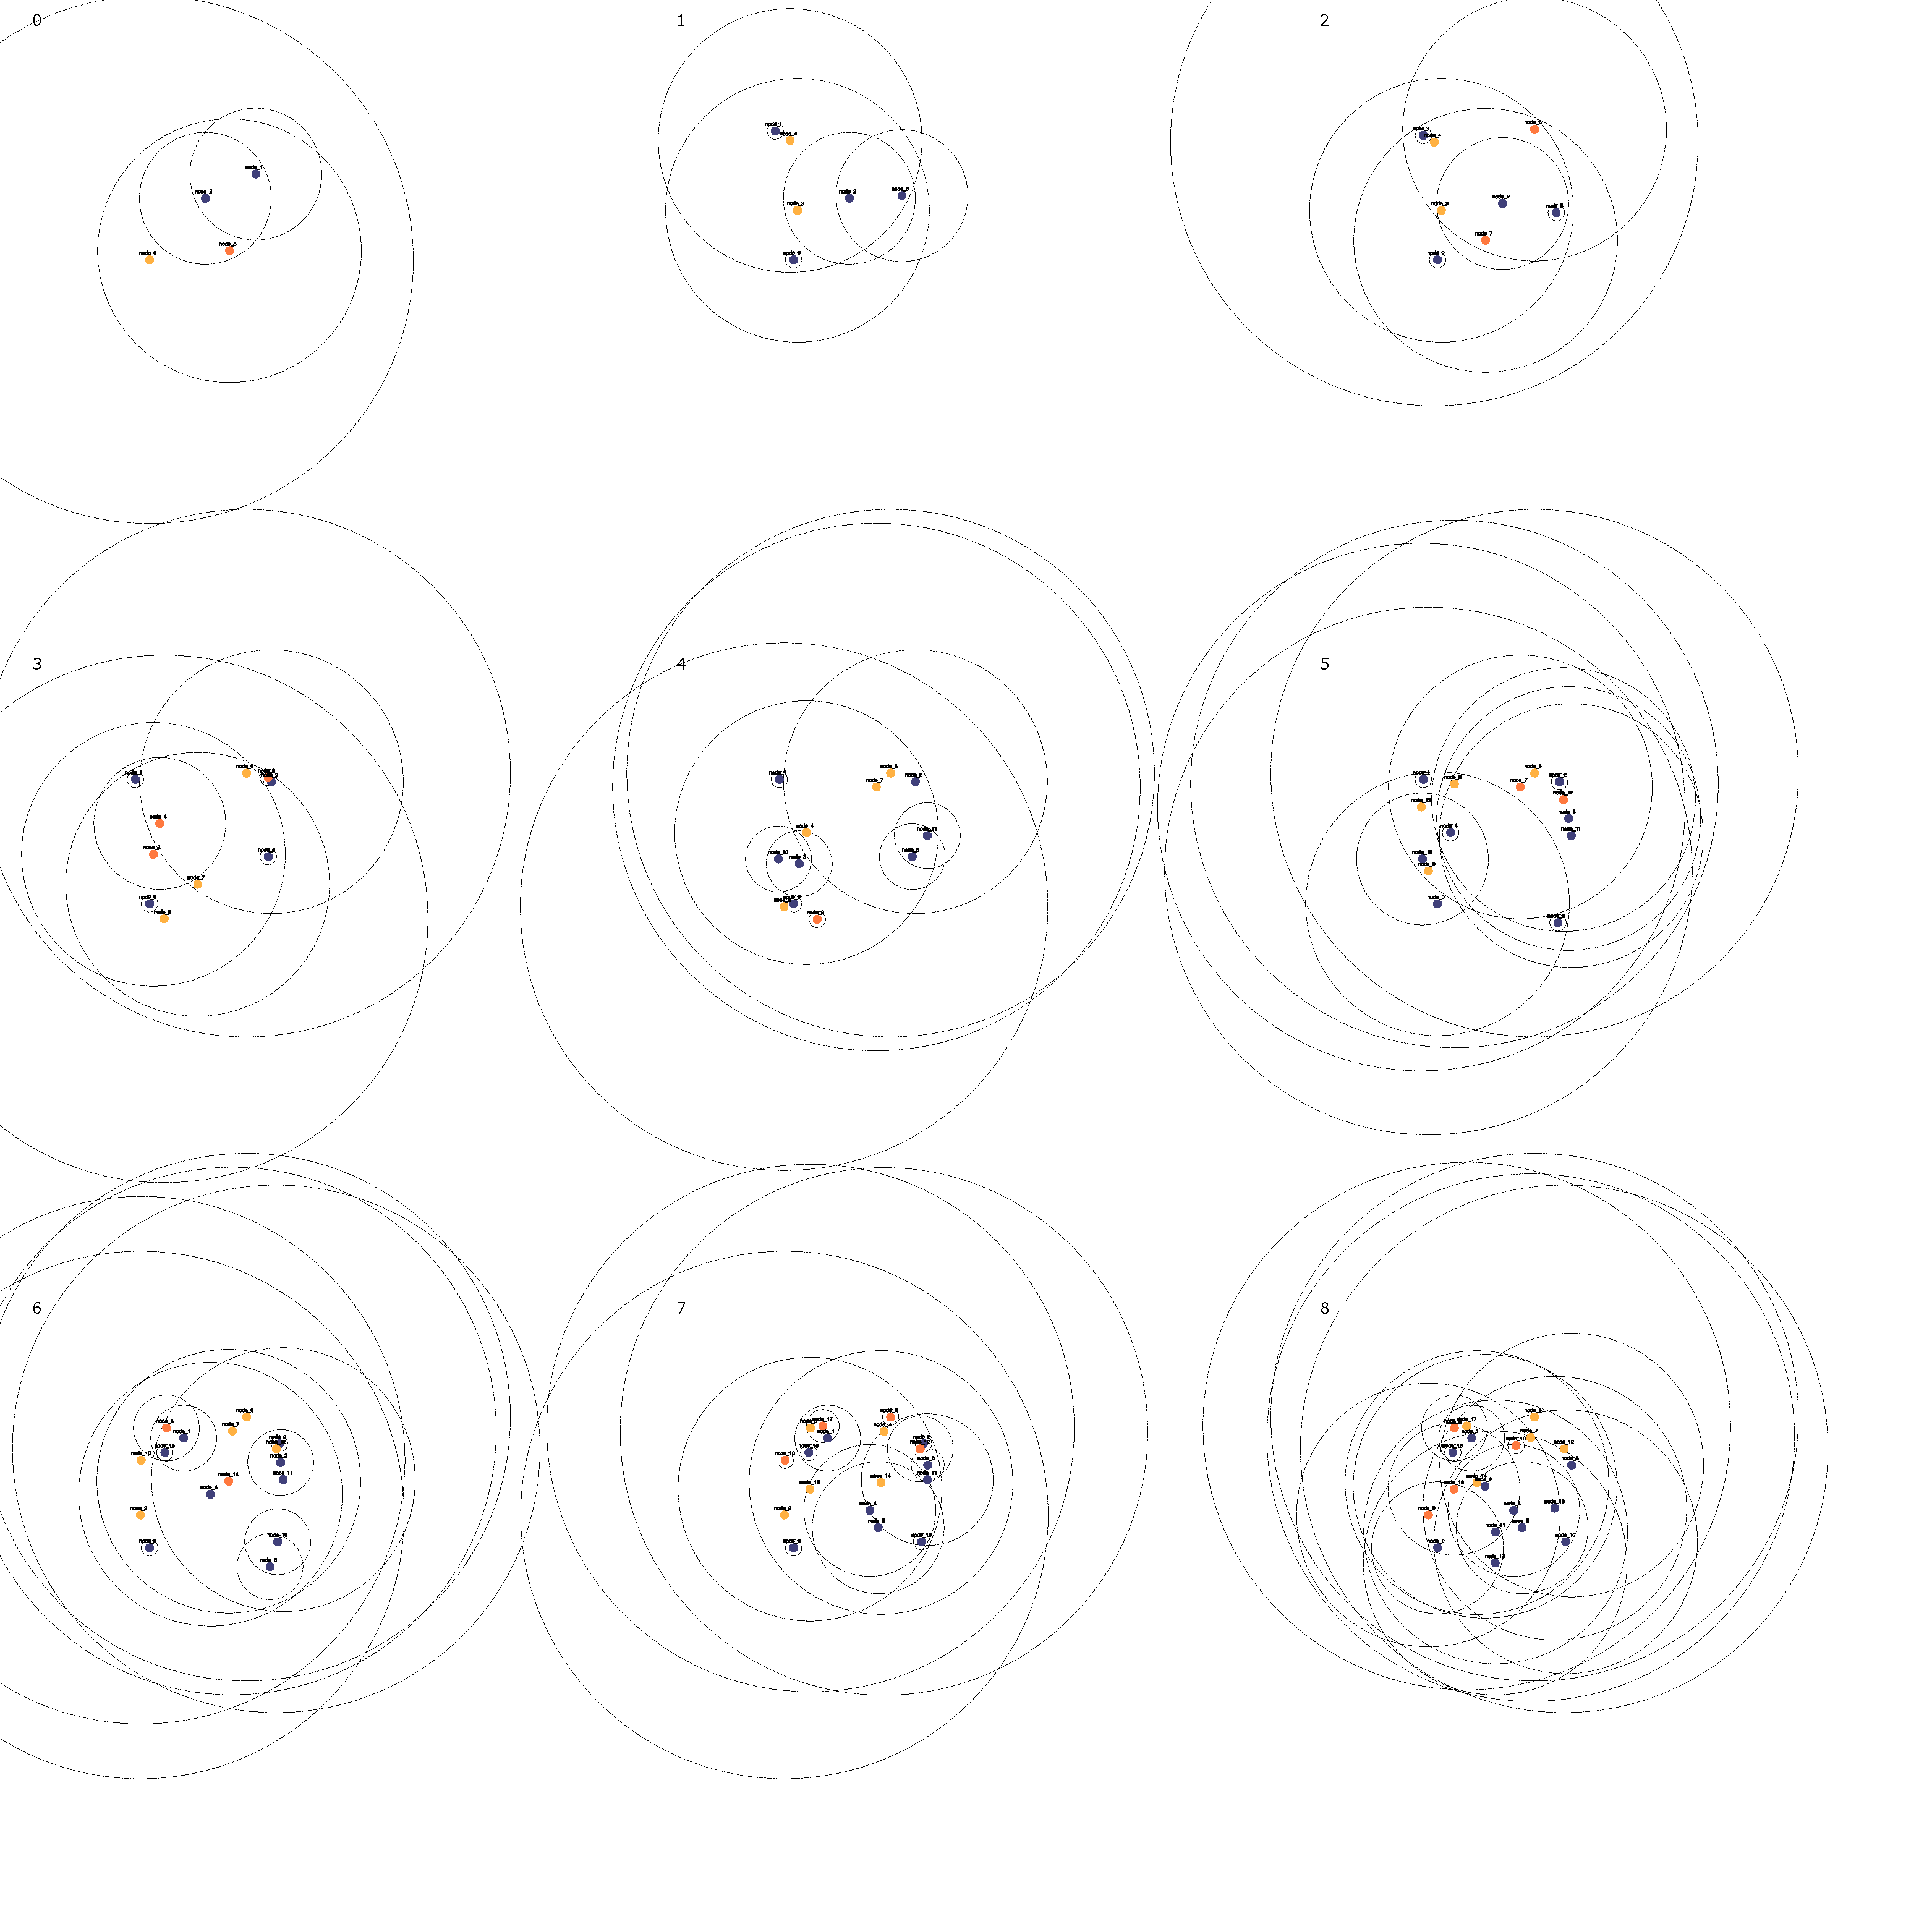
\includegraphics[width=350pt]{figures/LocarnoTreaties-RandomFinal}
\caption{Graphs of the system at each epoch, the levels are depicted in different colors.}
\label{fig:LocarnoTreaties-RandomFinal}
\end{figure}

\begin{figure}[!h] 
\centering
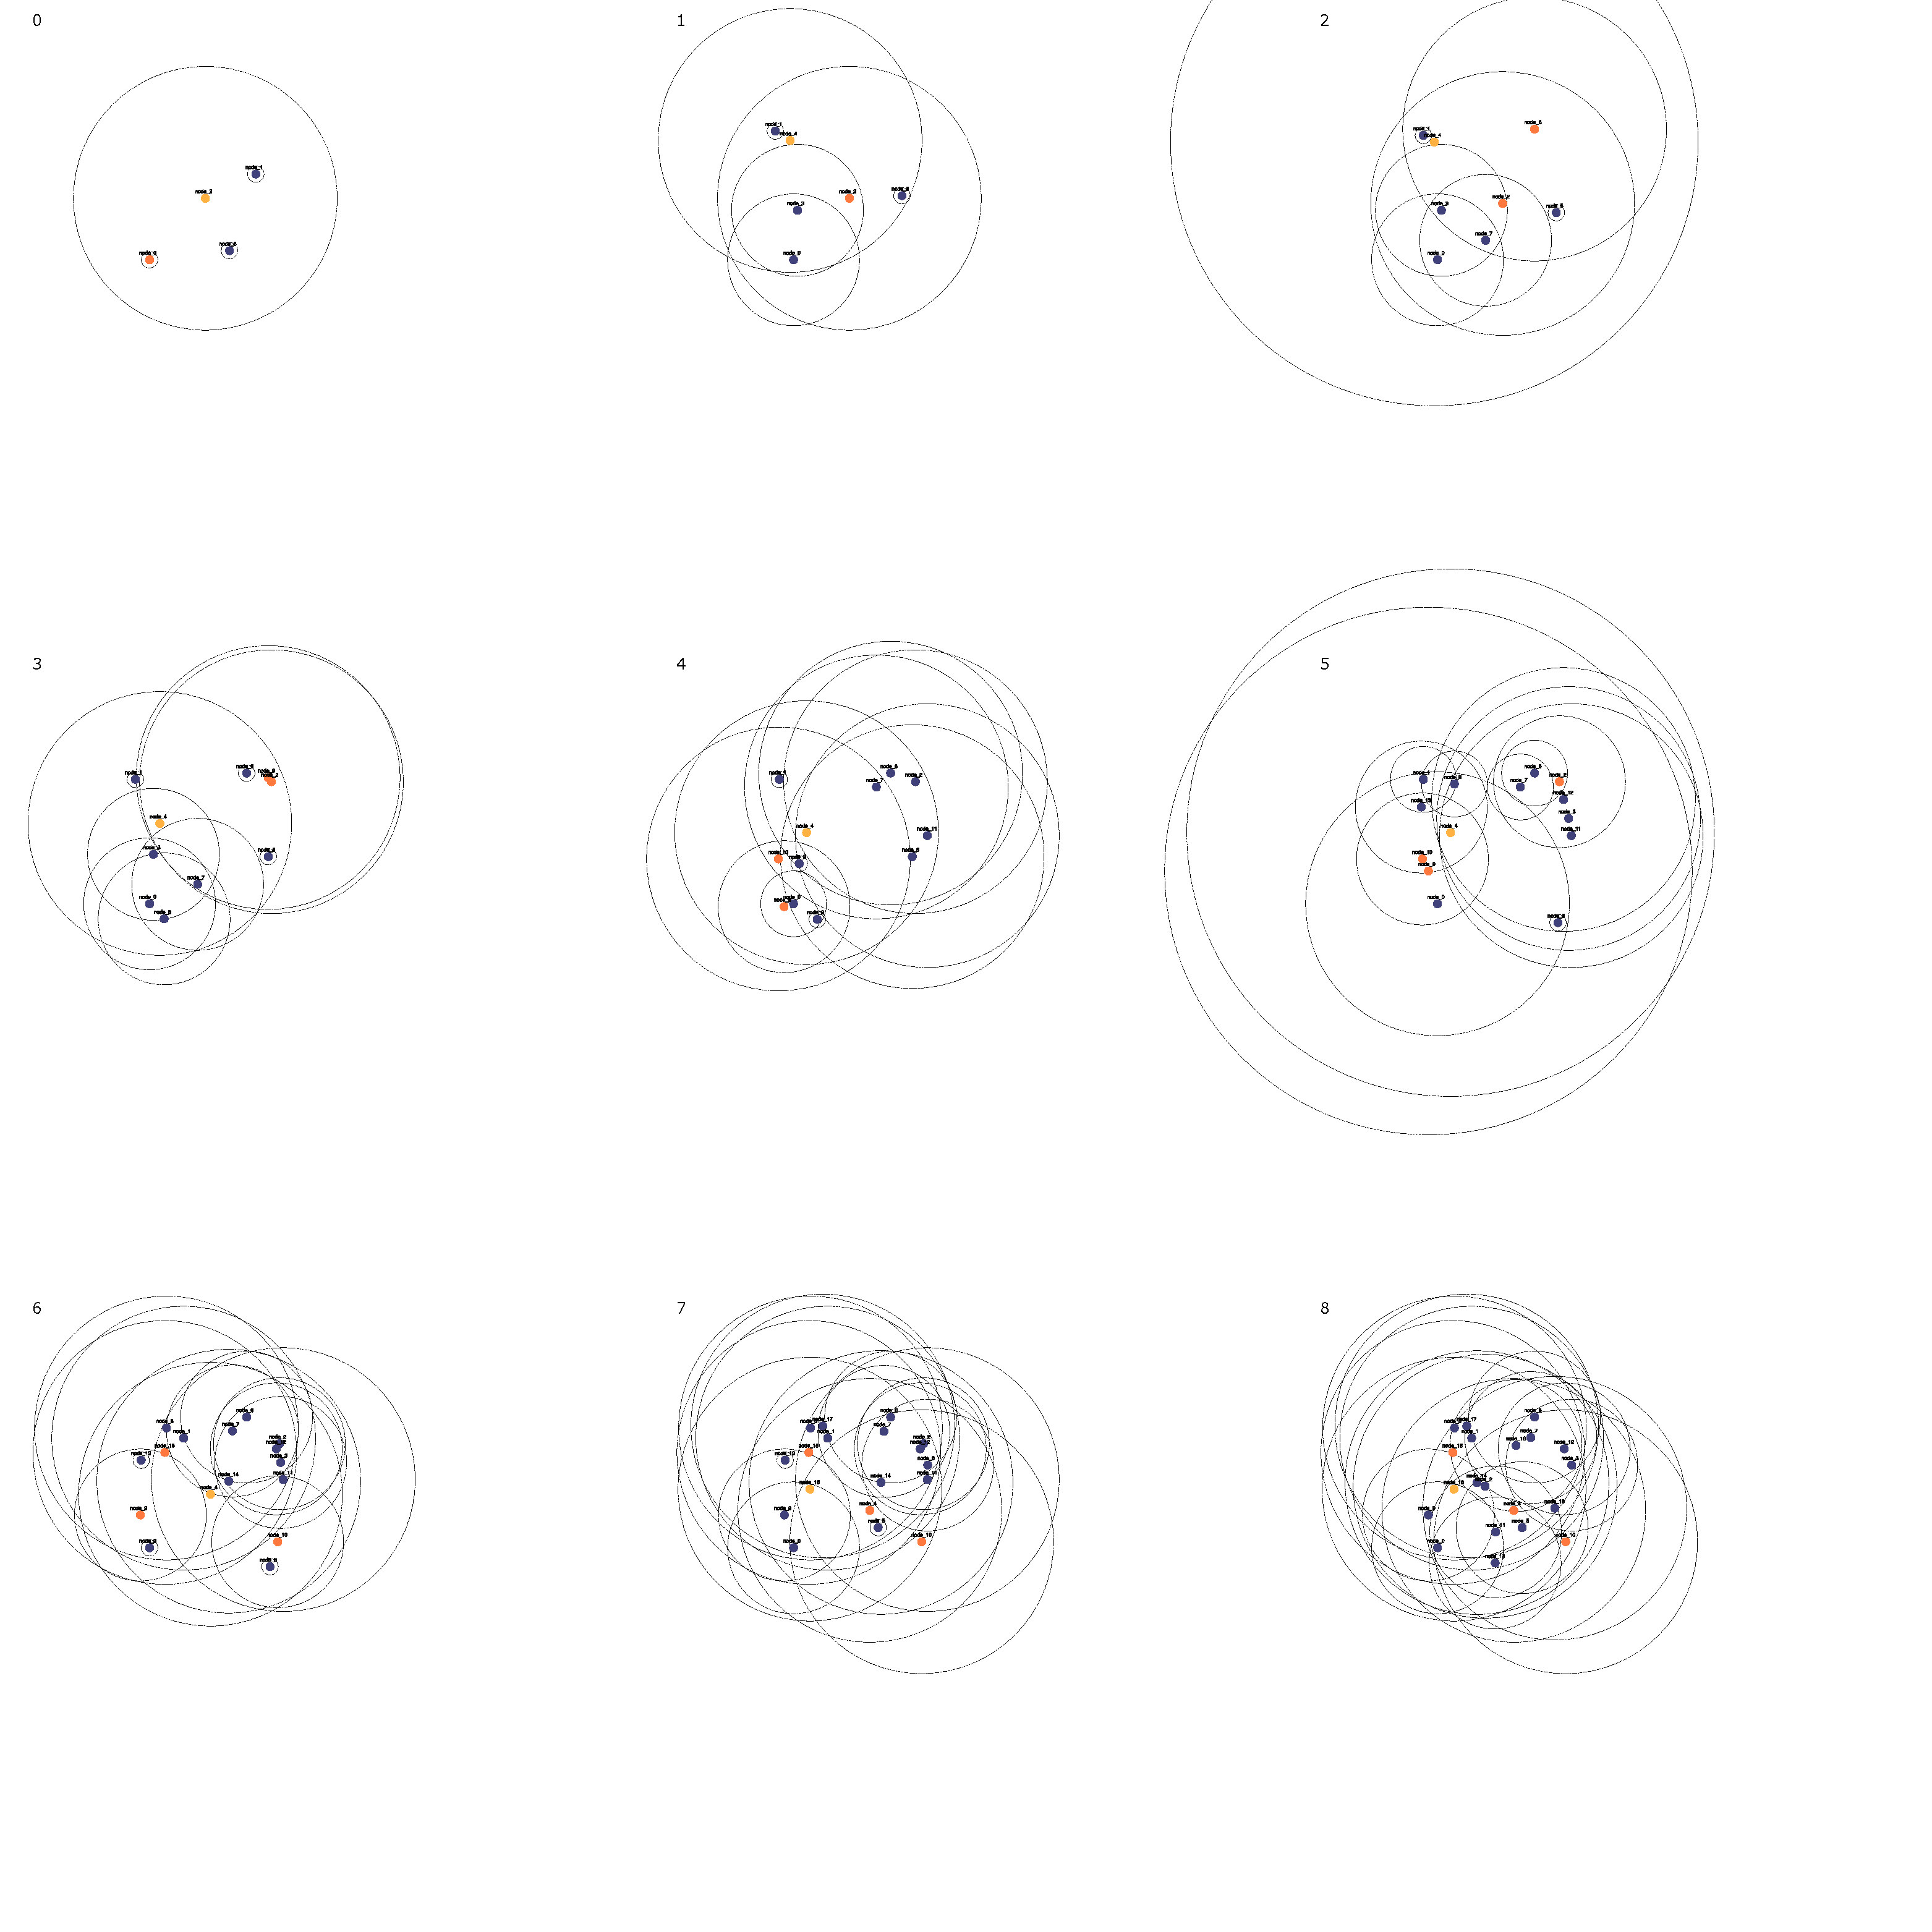
\includegraphics[width=500pt]{figures/LocarnoTreaties-LocarnoFinal}
\caption{Graphs of the system at each epoch, the levels are depicted in different colors.}
\label{fig:LocarnoTreaties-LocarnoFinal}
\end{figure}




\end{document}
